%!TEX program = xelatex
\documentclass[dvipsnames, svgnames,a4paper,11pt]{article}
% ----------------------------------------------------- 
%	加边框的命令
%	参考:https://tex.stackexchange.com/questions/531559/how-to-add-the-page-border-for-first-two-pages-in-latex
\usepackage{tikz}
\usetikzlibrary{calc}
\usepackage{eso-pic}
\AddToShipoutPictureBG{%
\begin{tikzpicture}[overlay,remember picture]
\draw[line width=0.6pt] % 边框粗细
    ($ (current page.north west) + (0.6cm,-0.6cm) $)
    rectangle
    ($ (current page.south east) + (-0.6cm,0.6cm) $); % 边框位置
\end{tikzpicture}}


\usepackage{xcolor}
\definecolor{c1}{HTML}{086173} % 目录颜色 原版为2752C9 紫灰色535AAA 蓝紫色0B0DB7 深蓝色070F94 湖绿色219394 松石灰绿086173
\definecolor{c2}{HTML}{E20129} % 引用颜色 原版\definecolor{c2}{RGB}{190,20,83} 橙色F24729

\usepackage{ctex}
\usepackage[top=28mm,bottom=28mm,left=15mm,right=15mm]{geometry}
\usepackage{hyperref} 
\hypersetup{
	colorlinks,
	linktoc = section, % 超链接位置,选项有section, page, all
	linkcolor = c1, % linkcolor 目录颜色
	citecolor = c1  % citecolor 引用颜色
}
\usepackage{amsmath,enumerate,multirow,float}
\usepackage{tabularx}
\usepackage{tabu}
\usepackage{subfig}
\usepackage{fancyhdr}
\usepackage{graphicx}
\usepackage{wrapfig}  
\usepackage{physics}
\usepackage{appendix}
\usepackage{amsfonts}

%
\usepackage{tcolorbox}
\tcbuselibrary{skins,breakable}
\newtcolorbox{tbox}[2][]{
    colframe=black!70!,
    breakable,
    enhanced,
	boxrule =0.5pt,
    title = {#2},
    fonttitle = \large\kaishu\bfseries,
	drop fuzzy shadow,
    #1
}
\newtcolorbox[auto counter,number within=section]{question}[1][]{
  top=2pt,bottom=2pt,arc=1mm,
  boxrule=0.5pt,
%   frame hidden,
  breakable,
  enhanced, %跨页后不会显示下边框
  coltitle=c1!80!gray,
  colframe=c1,
  colback=c1!3!white,
  drop fuzzy shadow,
  title={思考题~\thetcbcounter:\quad},
  fonttitle=\bfseries,
  attach title to upper,
  #1
}

% ---------------------------------------------------------------------
%	利用cleveref改变引用格式,\cref是引用命令
\usepackage{cleveref}
\crefformat{figure}{#2{\textcolor{c2}{Figure #1}}#3} % 图片的引用格式
\crefformat{equation}{#2{(\textcolor{c2}{#1})}#3} % 公式的引用格式
\crefformat{table}{#2{\textcolor{c2}{Table #1}}#3} % 表格的引用格式


% ---------------------------------------------------------------------
%	页眉页脚设置
\fancypagestyle{plain}{\pagestyle{fancy}}
\pagestyle{fancy}
\lhead{\kaishu 中山大学物理与天文学院电子技术实验\uppercase\expandafter{\romannumeral1}} % 左边页眉,学院 + 课程
\rhead{\kaishu 实验报告By黄罗琳} % 右边页眉,实验报告标题
\cfoot{\thepage} % 页脚,中间添加页码


% ---------------------------------------------------------------------
%	对目录、章节标题的设置
\renewcommand{\contentsname}{\centerline{\huge 目录}}
\usepackage{titlesec}
\usepackage{titletoc}
% \titleformat{章节}[形状]{格式}{标题序号}{序号与标题间距}{标题前命令}[标题后命令]
\titleformat{\section}{\centering\LARGE\songti}{}{1em}{}

% ---------------------------------------------------------------------
%   listing代码环境设置
\usepackage{listings}
\lstloadlanguages{python}
\lstdefinestyle{pythonstyle}{
backgroundcolor=\color{gray!5},
language=python,
frameround=tftt,
frame=shadowbox, 
keepspaces=true,
breaklines,
columns=spaceflexible,                   
basicstyle=\ttfamily\small, % 基本文本设置,字体为teletype,大小为scriptsize
keywordstyle=[1]\color{c1}\bfseries, 
keywordstyle=[2]\color{Red!70!black},   
stringstyle=\color{Purple},       
showstringspaces=false,
commentstyle=\ttfamily\scriptsize\color{green!40!black},%注释文本设置,字体为sf,大小为smaller
tabsize=2,
morekeywords={as},
morekeywords=[2]{np, plt, sp},
numbers=left, % 代码行数
numberstyle=\it\tiny\color{gray}, % 代码行数的数字字体设置
stepnumber=1,
rulesepcolor=\color{gray!30!white}
}




% ---------------------------------------------------------------------
%	其他设置
\def\degree{${}^{\circ}$} % 角度
\graphicspath{{./images/}} % 插入图片的相对路径
\allowdisplaybreaks[4]  %允许公式跨页 
\usepackage{lipsum}
\usepackage{adjustbox}
\usepackage{amsmath}
\usepackage{pgfplots}
%\usepackage{mathrsfs} % 字体
%\captionsetup[figure]{name=Figure} % 图片形式
%\captionsetup[table]{name=Table} % 表格形式
\begin{document}
	
	% 实验报告封面	
	% 顶栏
	\begin{table}
		\renewcommand\arraystretch{1.7}
		\begin{tabularx}{\textwidth}{
				|X|X|X|X
				|X|X|X|X|}
			\hline
			\multicolumn{2}{|c|}{预习报告}&\multicolumn{2}{|c|}{实验记录}&\multicolumn{2}{|c|}{分析讨论}&\multicolumn{2}{|c|}{总成绩}\\
			\hline
			\LARGE25 & & \LARGE25 & & \LARGE30 & & \LARGE80 & \\
			\hline
		\end{tabularx}
	\end{table}
	% ---
	
	% 信息栏
	\begin{table}
		\renewcommand\arraystretch{1.7}
		\begin{tabularx}{\textwidth}{|X|X|X|X|}
			\hline
			年级、专业: & 2022级 物理学 &组号: & \\
			\hline
			姓名: & 黄罗琳、王显   & 学号: &22344001、2234002   \\
			\hline
			实验时间: & 2024/5/29 & 教师签名: & \\
			\hline
		\end{tabularx}
	\end{table}
	% ---
	
	% 大标题
	\begin{center}
		\LARGE ET13\quad 整流滤波与稳压电路
	\end{center}
	% ---
	
	% 注意事项
	
	% 基本
	\textbf{【实验报告注意事项】}
	\begin{enumerate}
		\item 实验报告由三部分组成:
		\begin{enumerate}
			\item 预习报告:课前认真研读实验讲义,弄清实验原理;实验所需的仪器设备、用具及其使用、完成课前预习思考题;了解实验需要测量的物理量,并根据要求提前准备实验记录表格(可以参考实验报告模板,可以打印)。\textcolor{red}{\textbf{(20分)}}
			\item 实验记录:认真、客观记录实验条件、实验过程中的现象以及数据。实验记录请用珠笔或者钢笔书写并签名(\textcolor{red}{\textbf{用铅笔记录的被认为无效}})。\textcolor{red}{\textbf{保持原始记录,包括写错删除部分,如因误记需要修改记录,必须按规范修改。}}(不得输入电脑打印,但可扫描手记后打印扫描件);离开前请实验教师检查记录并签名。\textcolor{red}{\textbf{(30分)}}
			\item 数据处理及分析讨论:处理实验原始数据(学习仪器使用类型的实验除外),对数据的可靠性和合理性进行分析;按规范呈现数据和结果(图、表),包括数据、图表按顺序编号及其引用;分析物理现象(含回答实验思考题,写出问题思考过程,必要时按规范引用数据);最后得出结论。\textcolor{red}{\textbf{(30分)}}
		\end{enumerate}
		\textbf{实验报告就是将预习报告、实验记录、和数据处理与分析合起来,加上本页封面。\textcolor{red}{(80分)}}
		\item 每次完成实验后的一周内交\textbf{实验报告}(特殊情况不能超过两周)。
		
	\end{enumerate}
	
	% 安全
	\textbf{【实验安全注意事项】}	
	\begin{enumerate}
		\item 由于变压器输出没有限流保护,接线时要注意不要短路;
		\item 用示波器测量时,注意两个通道探头的地线要共地;
		\item 用示波器测量纹波大小时,可以先采用直流耦合,获取直流分量的平均值,再采用交流耦合,观测纹波的波动范围;
		\item 选择和调节负载电阻时,注意不要使负载电流过大;
		
	\end{enumerate}
	
	% 目录
	\clearpage
	\tableofcontents
	\clearpage
	% ---
	
	
	
	% 预习报告	
	
	% 小标题
	\setcounter{section}{0}
	\section{ET13整流滤波与稳压电路 \quad\heiti 预习报告}
	% ---
	
	% 实验目的
	\subsection{实验目的}
	\begin{enumerate}
		\item 比较半波整流与桥式整流的特点。
		\item 了解稳压电路的组成和稳压作用。
		\item 熟悉集成三端可调稳压器的使用。
		\item 掌握直流稳压电源主要参数测试方法。
	\end{enumerate}
	% ---
	
	% 仪器用具
	\subsection{仪器用具}
	\begin{table}[htbp]
		\centering
		\renewcommand\arraystretch{1.6}
		% \setlength{\tabcolsep}{10mm}
		\begin{tabular}{p{0.05\textwidth}|p{0.20\textwidth}|p{0.05\textwidth}|p{0.5\textwidth}}
			\hline
			编号 & 仪器用具名称 & 数量 & 主要参数(型号,测量范围,测量精度等) \\
\hline
1 & 模拟电路实验箱 & 1 &  \\
2 & 数字万用表 & 1 & RIGOL DM3058E \\
3 & 函数信号发生器 & 1 & RIGOL DG4162 \\
4 & 双踪示波器 & 1 & RIGOL DS1104Z PLUS \\
5 & 直流稳压电源 & 1 & RIGOL DP831 \\
6 & 导线 & 若干 & 无 \\
			\hline
		\end{tabular}
	\end{table}
	% ---
	
	% 原理概述
	\subsection{原理概述}
	\begin{enumerate}
		\item 半波整流电路
		  \begin{figure}[{H}]
			\centering
			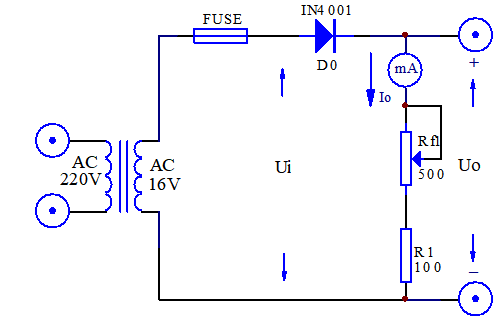
\includegraphics[width=0.4\linewidth]{半波整流.png}
			\caption{实验电路}
			\label{}
		  \end{figure}
		  220V、 50Hz 的市电交流正弦信号经过变压器降压后的幅度有效值约 16V,频率 50Hz。经过整流二极管后,在负载 Rf+R1 上,得到一个脉动电压,由于二极管的单向导通作用,只有 14V 交流信号的正半周可以通过载,负半周被二极管阻断,无法通过。

	    \item 全波整流(桥式整流)电路
	    \begin{figure}[{H}]
			\centering
			\includegraphics[width=0.4\linewidth]{桥.png}
			\caption{实验电路}
			\label{}
		\end{figure}
		半波整流电路简单,但是电源利用效率低,电压波动大。通过 4 只二极管的巧妙连接,可以实现全波整流。电源正半周通过 D4,负载, D3 流通,负半周通过 D1,负载, D2 流通,这样电源的正负半周都作用到了负载上,在负载上得到上正下负的直流脉动电压,提升了电源利用效率,减少了输出电压波动。这 4 只二极管组成的全波整流电路,也称之为整流桥,这种整流方法称之为桥式整流。
		\item 电容滤波电路
		\begin{figure}[{H}]
			\centering
			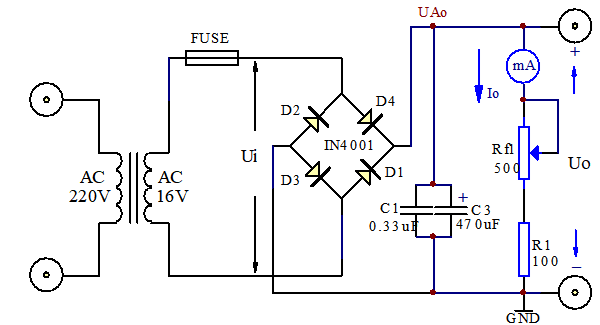
\includegraphics[width=0.4\linewidth]{电容.png}
			\caption{实验电路}
			\label{}
		\end{figure}
		无论半波整流还是全波整流的输出电压都是脉动的,为了得到输出电压相对稳定的平滑的直流电,可通过滤除交流成分的滤波电路来实现。利用电容的充放电特性组建的电容滤波电路是最常用的滤波电路。当整流后脉动电压值大于电容两端电压时给电容充电,直到电压峰值,当整流后的脉动电压值低于电容电压时,电容放电向负载提供电流,电容电压下降速度按指数规律(参考一阶电路)。如此循环往复,使输出电压在较小范围内波动,这个波动范围也成为电源纹波。
		\item 稳压管并联稳压电路
		\begin{figure}[{H}]
			\centering
			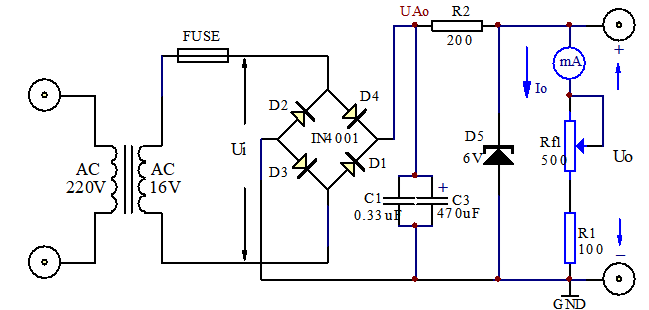
\includegraphics[width=0.4\linewidth]{稳压管.png}
			\caption{实验电路}
			\label{}
		\end{figure}
		电容滤波电路可以把整流后的脉动电压限制在某个固定值附近波动,但是电压波动的平均值取决于变压器输出,也和滤波电容与负载电阻的大小相关,不能随意调整。如果用电设备需要在输入电压波动时得到稳定的直流电压供应,就需要不同结构的稳压电路提供稳压电源。

		此时可以利用稳压二极管的反向稳压特性,把分压限流电阻R2和稳压二极管D5并联接入滤波电容的两端,就可以在稳压二极管两端得到稳定的电压输出。

稳压管并联稳压电路受负载变化影响较大,当负载变化时,负载与R2的分压也会发生变化,当负载电阻变小时,负载分压降低会导致稳压管无法稳压。

		\item 三端集成稳压器电路

		\begin{figure}[{H}]
			\centering
			\includegraphics[width=0.4\linewidth]{三.png}
			\caption{实验电路}
			\label{}
		\end{figure}
		常用的三端集成稳压器是78XX和79XX系列,78XX是正电压稳压器,79XX是负电压稳压器。XX是设定好的稳压电压值。以78XX系列为例,7805,输出电压5V,7812,输出电压12V。
	\end{enumerate}
	% ---
	
	
	
	% 实验前思考题
	\subsection{实验预习题}
	
	% 思考题1
	\begin{question}
	RC一阶电路时间常数对电容放电曲线的影响;
	\end{question}
时间常数 $\tau$ 定义为:
\[
\tau = R \cdot C
\]

电容放电时,电压 $V(t)$ 随时间 $t$ 的变化可以表示为:
\[
V(t) = V_0 e^{-\frac{t}{\tau}}
\]

其中,$V_0$ 是初始电压。

\begin{itemize}
    \item 当 $t = \tau$ 时,$V(t) = V_0 e^{-1} \approx 0.368 V_0$
    \item 当 $t = 2\tau$ 时,$V(t) = V_0 e^{-2} \approx 0.135 V_0$
    \item 当 $t = 3\tau$ 时,$V(t) = V_0 e^{-3} \approx 0.050 V_0$
    \item 当 $t = 5\tau$ 时,$V(t) \approx 0$
\end{itemize}


	% 思考题2
	\begin{question}
		稳压二极管特性
	\end{question}
稳压二极管(也称齐纳二极管)是一种特殊类型的二极管,它在反向击穿区域具有稳定的电压特性。以下是稳压二极管的主要特性和工作原理:

稳压二极管在正向偏置时的行为与普通二极管类似,但在反向偏置时,当反向电压达到某一特定值(称为击穿电压或齐纳电压 $V_Z$)时,二极管会进入击穿区域,并且在这一区域内电压几乎保持不变。

在击穿区域,稳压二极管的电压基本恒定,即使通过二极管的电流有较大变化。这种特性使得稳压二极管非常适合用于电压稳压和电压参考电路。

稳压二极管的击穿机制主要包括齐纳击穿和雪崩击穿:

\begin{itemize}
    \item \textbf{齐纳击穿}:在低于 5V 的反向击穿电压下,电场强度足够高以致使价带中的电子跃迁到导带,形成击穿电流。
    \item \textbf{雪崩击穿}:在高于 5V 的反向击穿电压下,由于电场较弱,载流子通过碰撞电离产生大量电子和空穴对,形成击穿电流。
\end{itemize}

稳压二极管常用于简单的电压稳压电路中,以提供稳定的输出电压。当输入电压 $V_\text{in}$ 大于齐纳电压 $V_Z$ 时,输出电压 $V_\text{out}$ 会稳定在 $V_Z$ 附近。

	% 思考题3
	\begin{question}
		电源效率的计算方法
	\end{question}
电源的效率用电源的输出功率除以电源的总功率。

输出功率 P 输=UI(U 是电源的输出电压也叫外电压、路端电压)

电源总功率 P 总=EI(E 是电源的电动势)

效率=P 输/P 总,一般比值换成百分比
	% ---
	
	
	
	% 实验记录	
	\clearpage
	
	% 顶栏
	\begin{table}
		\renewcommand\arraystretch{1.7}
		\centering
		\begin{tabularx}{\textwidth}{|X|X|X|X|}
			\hline
			专业: & 物理学 & 年级: & 2022级 \\
			\hline
			姓名: &黄罗琳、王显  & 学号: &22344001、22344002 \\
			\hline
			室温: & 25℃ & 实验地点: & A522 \\
			\hline
			学生签名:& 见\textbf{附件}部分 & 评分: &\\
			\hline
			实验时间:& 2024/6/12 & 教师签名:&\\
			\hline
		\end{tabularx}
	\end{table}
	% ---
	
	% 小标题
	\section{ET13整流滤波与稳压电路  \quad\heiti 实验记录}
	% ---
	
	% 实验过程记录
	\subsection{实验内容、步骤与结果}
	\subsubsection{观察实验原始输出波形}
	\begin{figure}[{H}]
		\centering
		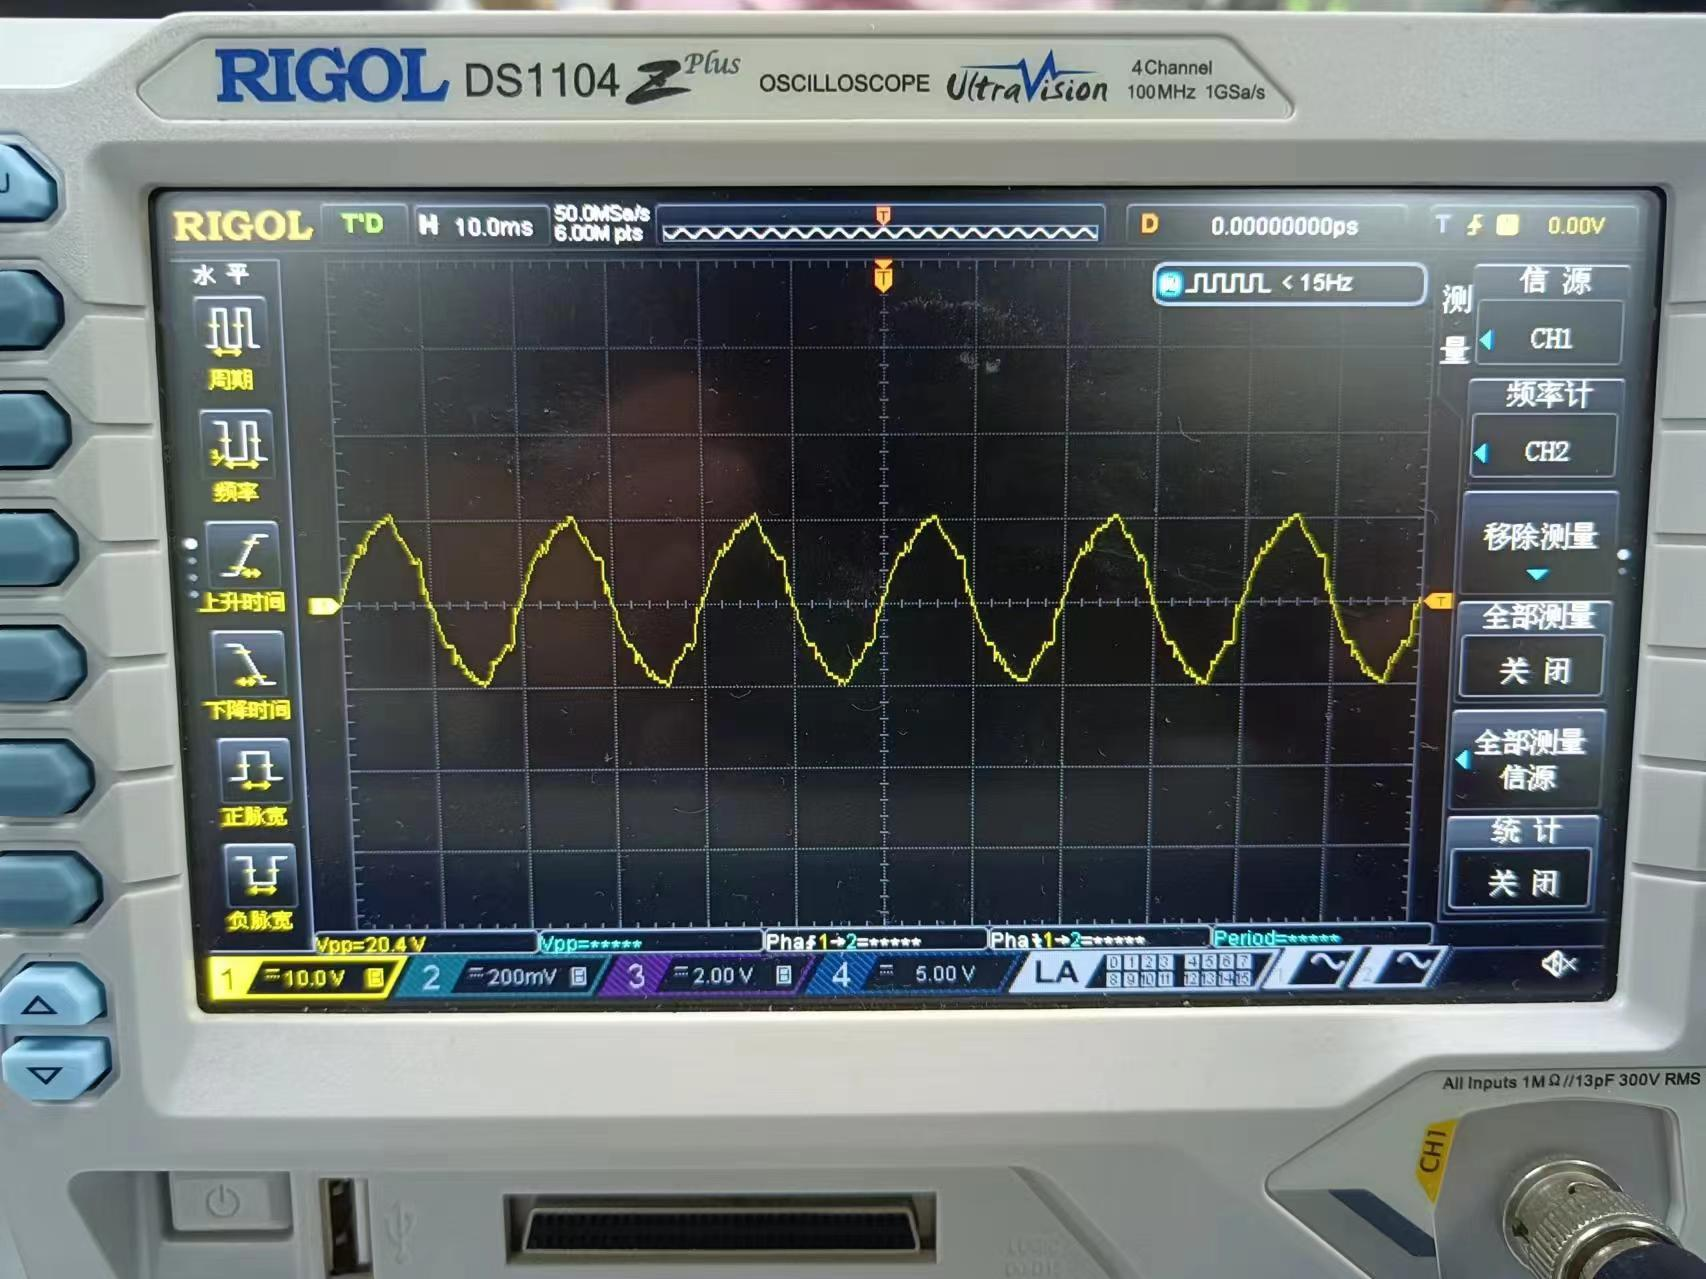
\includegraphics[width=0.4\linewidth]{原始.jpg}
		\caption{实验电路原始输出波形}
		\label{}
	\end{figure}
	%
	\subsubsection{搭建半波整流电路,用示波器观测和记录输出波形}
	\begin{figure}[{H}]
		\centering
		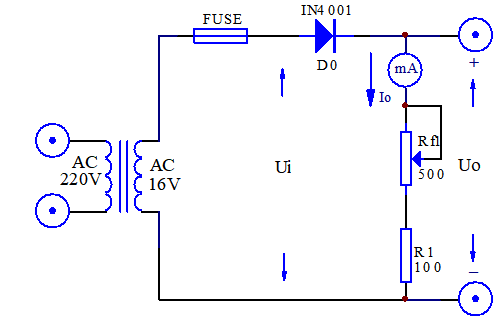
\includegraphics[width=0.4\linewidth]{半波整流.png}
		\caption{实验电路图}
		\label{}
	\end{figure}
	电路参数如图:14V(AC)  
	\begin{figure}[{H}]
		\centering
		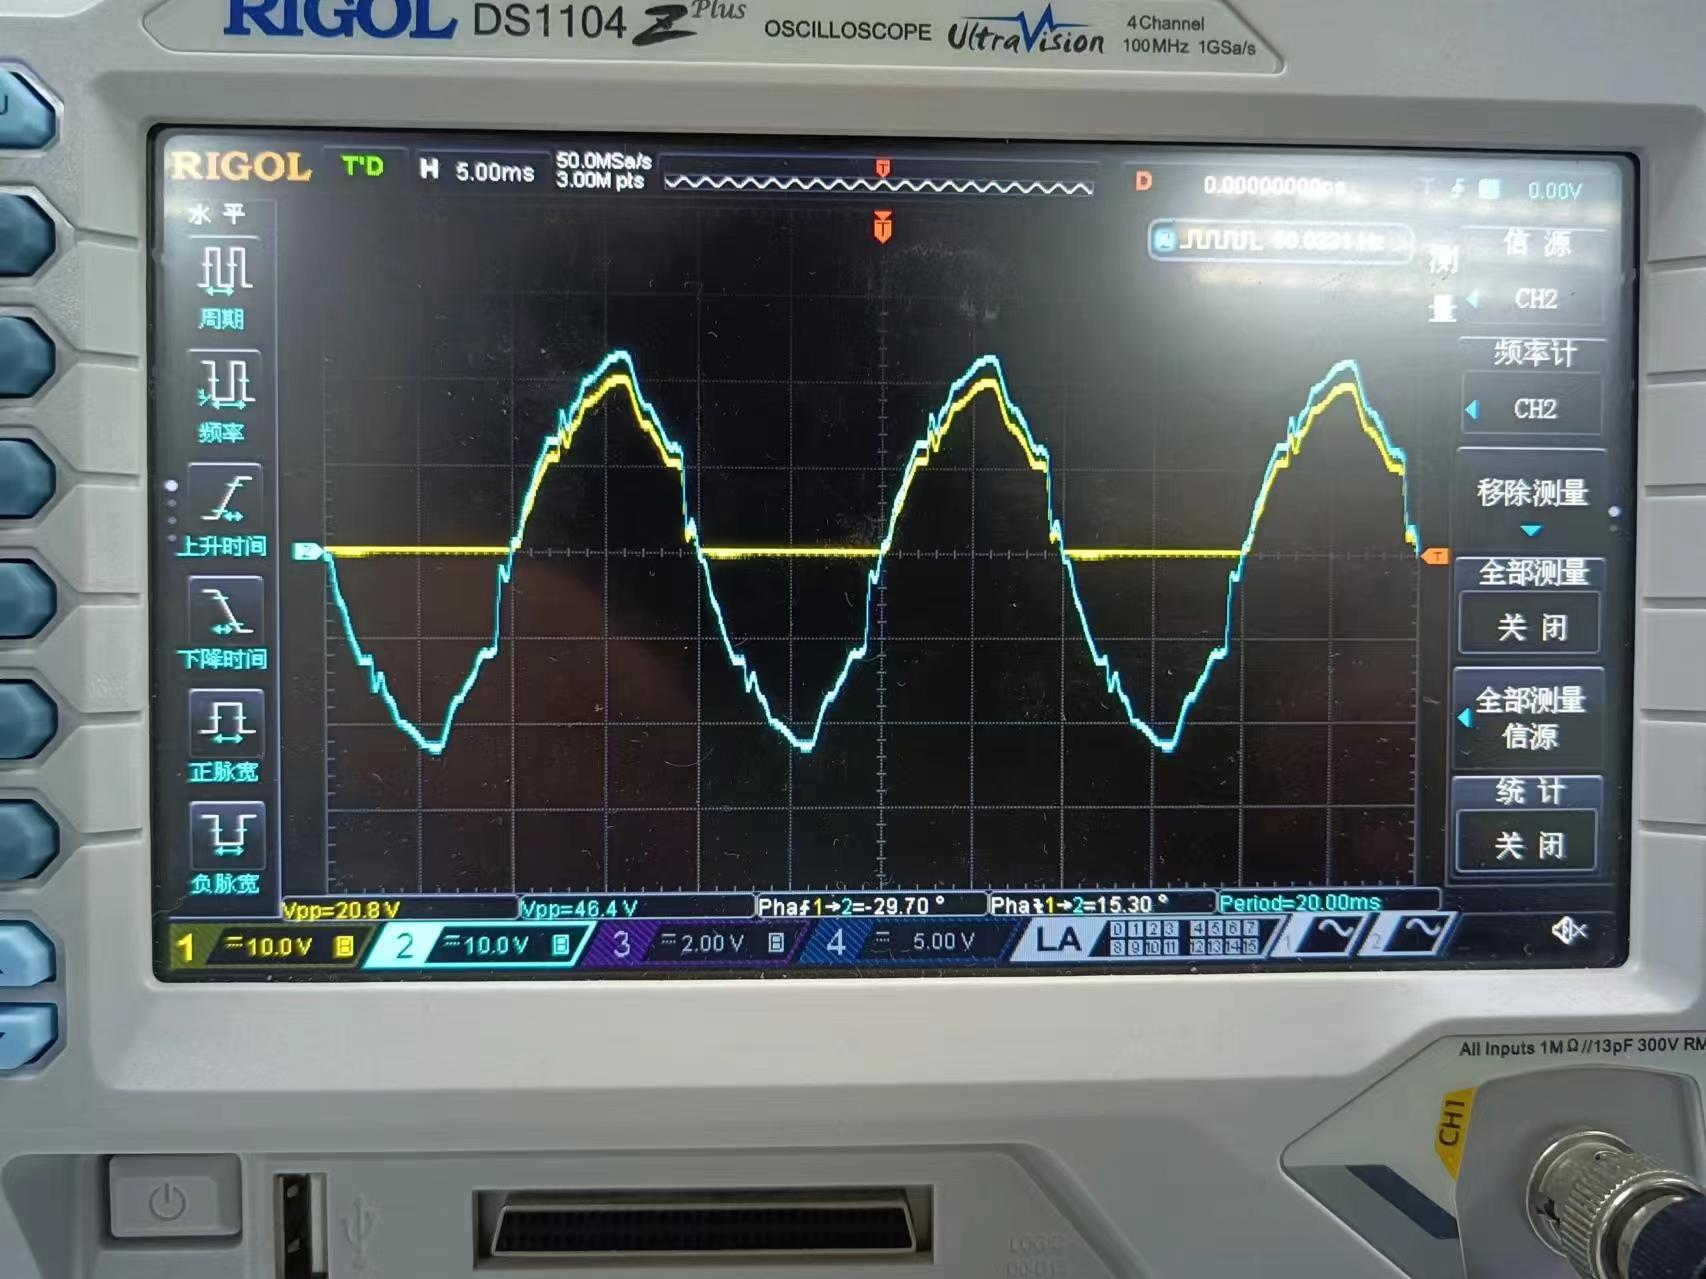
\includegraphics[width=0.4\linewidth]{半波比较.jpg}
		\caption{整流图像}
		\label{}
	\end{figure}
	\begin{figure}[{H}]
		\centering
		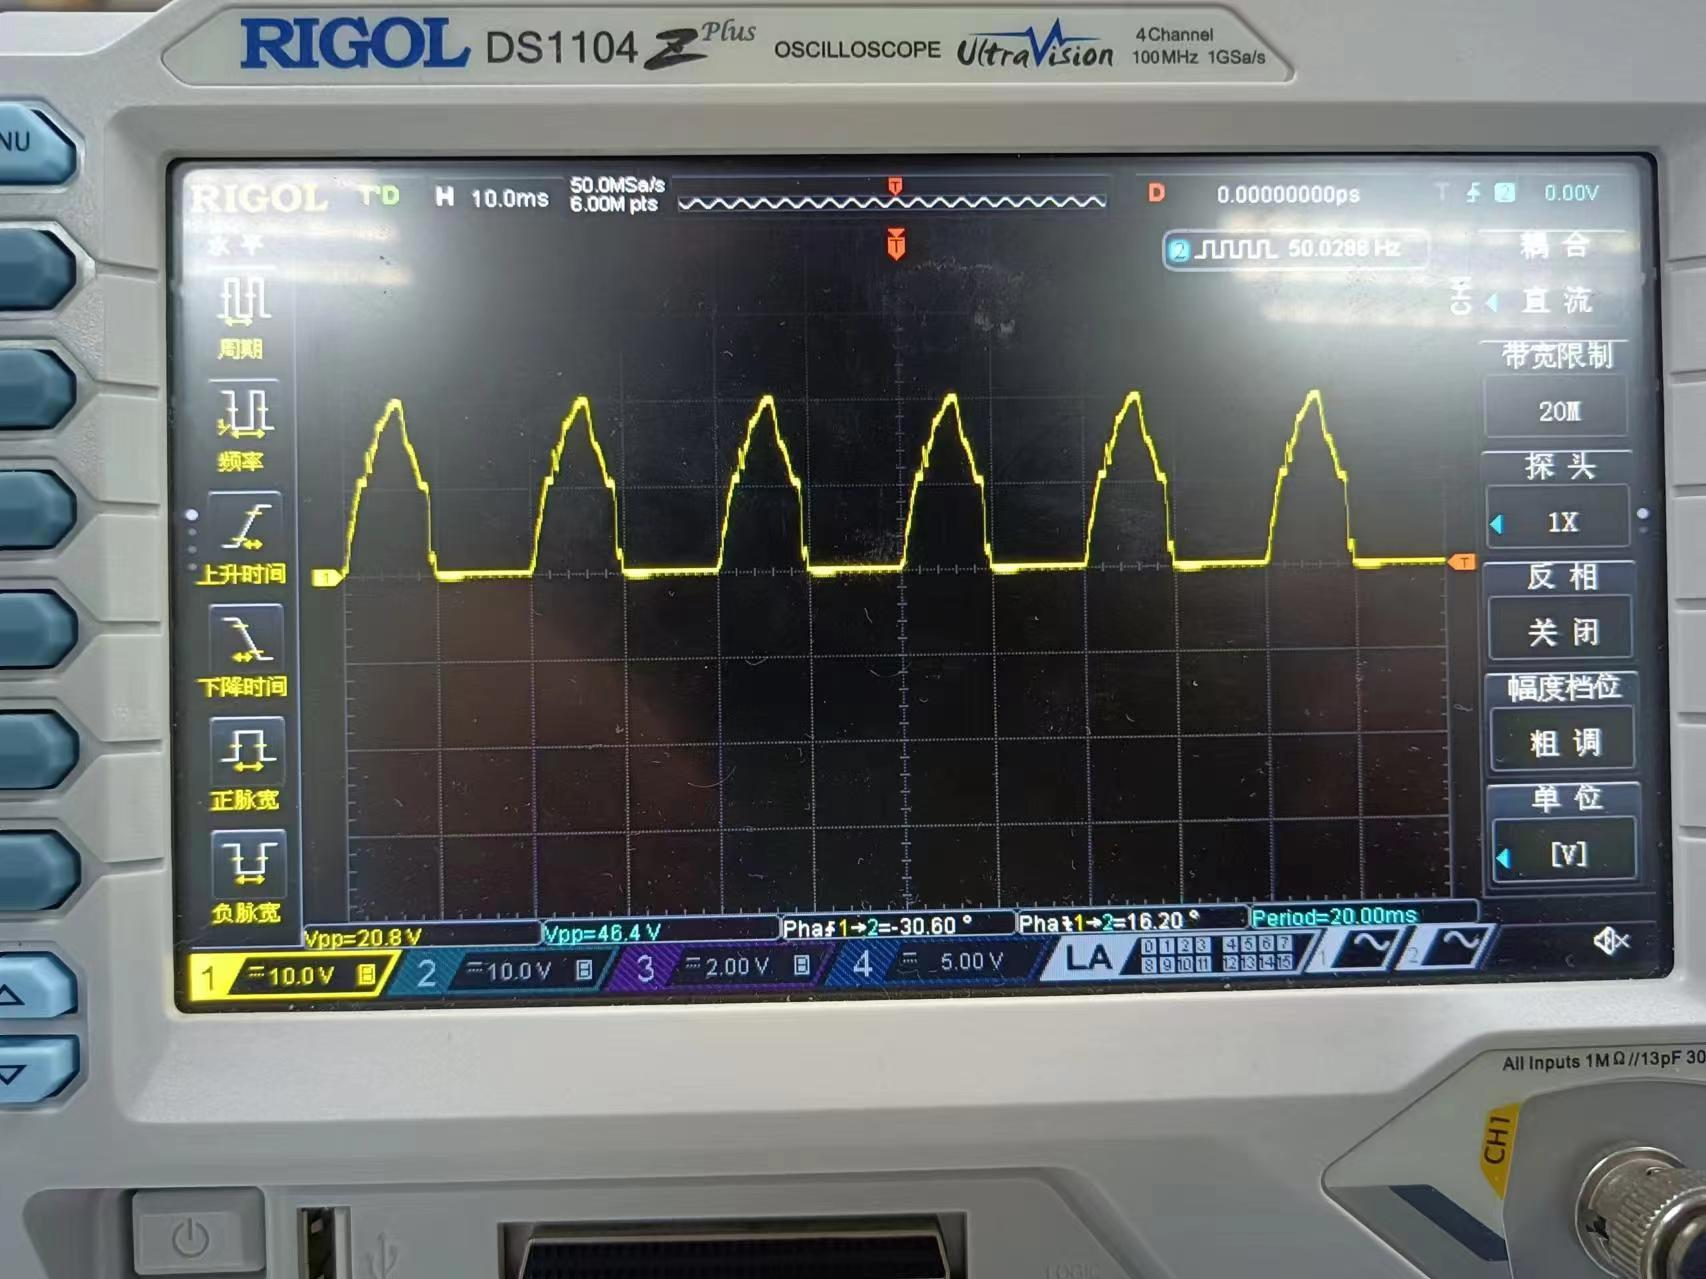
\includegraphics[width=0.4\linewidth]{半波单独.jpg}
		\caption{整流图像}
		\label{}
	\end{figure}
	%
	\subsubsection{搭建全波整流电路,用示波器观测和记录输出波形}
\begin{figure}[{H}]
	\centering
	\includegraphics[width=0.4\linewidth]{桥.png}
	\caption{实验电路}
	\label{}
\end{figure}
电路参数如图:14V(AC)  
\begin{figure}[{H}]
	\centering
	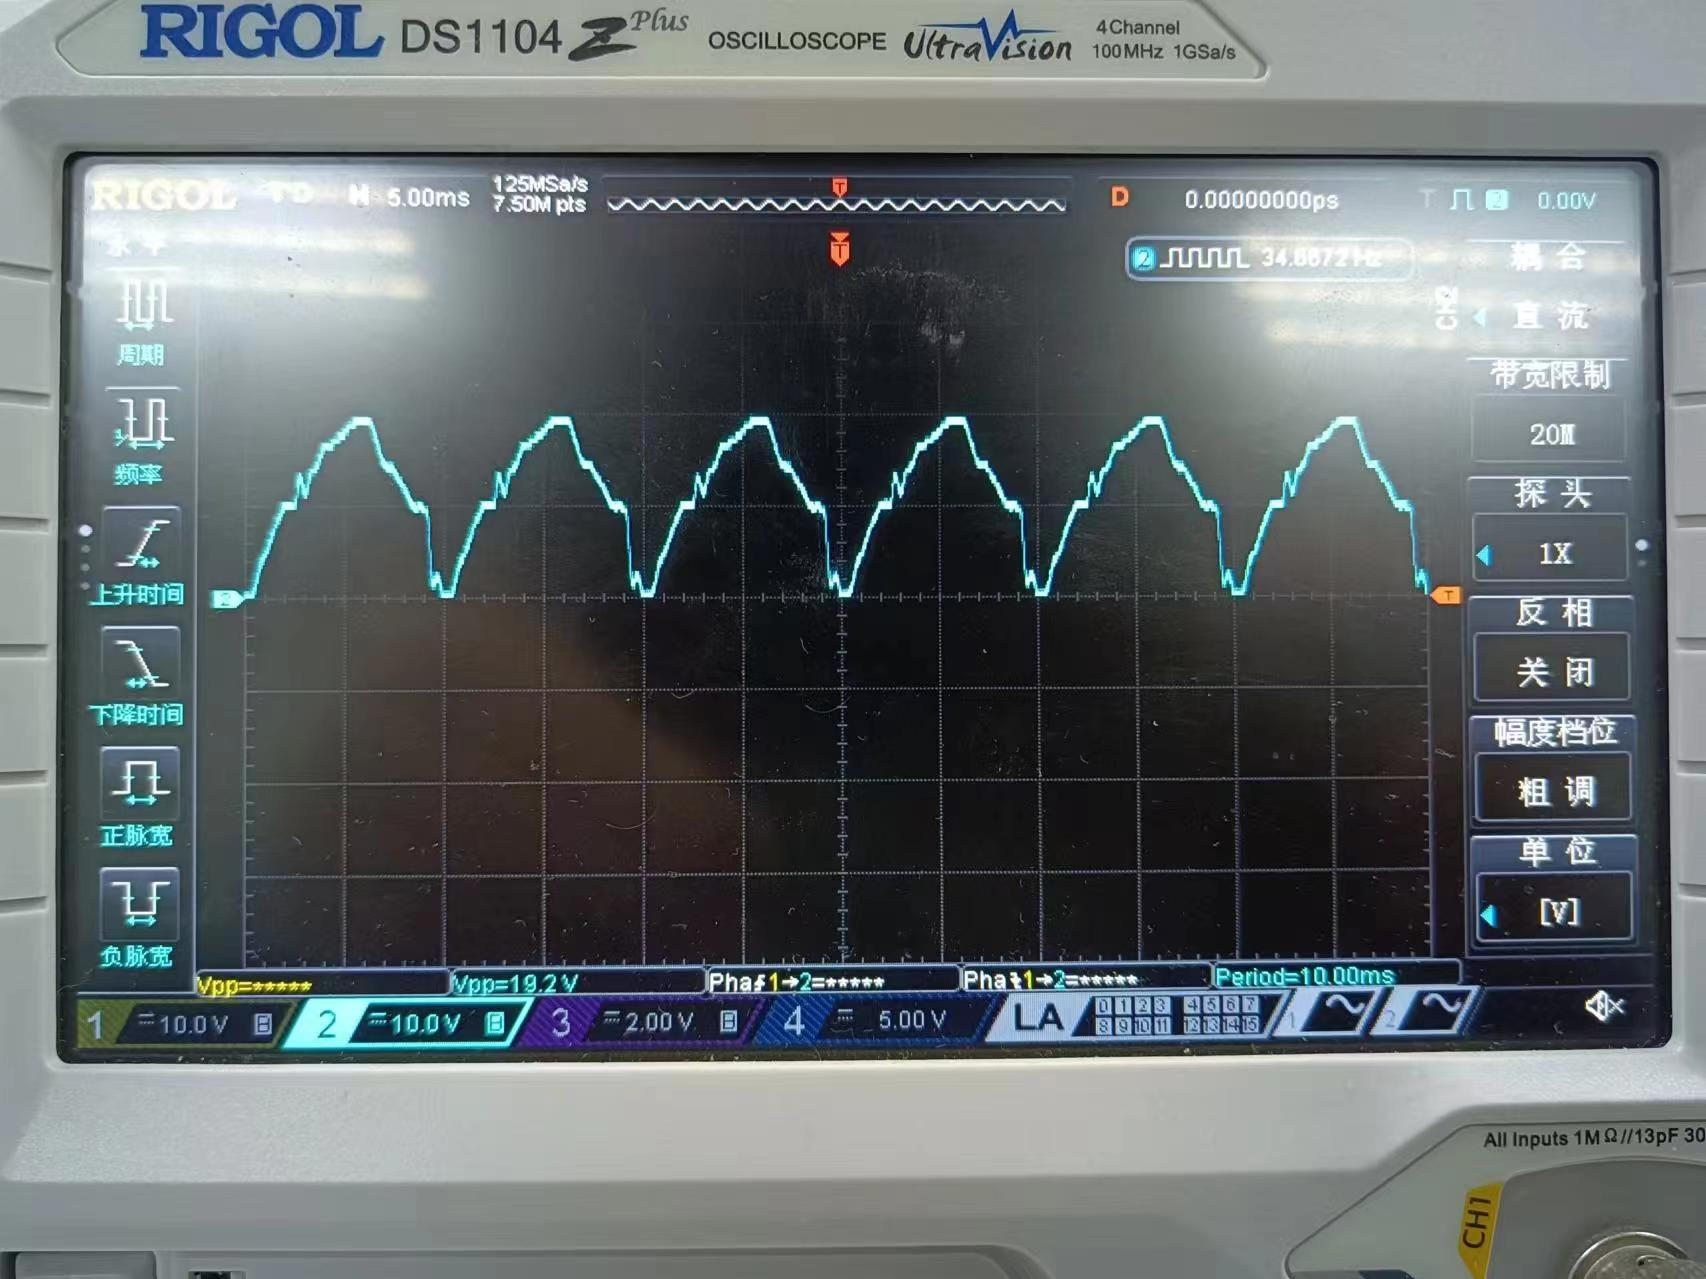
\includegraphics[width=0.4\linewidth]{全波单独.jpg}
	\caption{整流图像}
	\label{}
\end{figure}
\subsubsection{在以上两种整流电路中,加入滤波电容,用示波器观测和记录输出波形;调整滤波电容和负载电阻,观测和记录输出纹波的变化规律}
\begin{enumerate}
	\item 半波整流 
	
	实验参数:$200\Omega\quad 470\mu F$
	\begin{figure}[{H}]
		\centering
		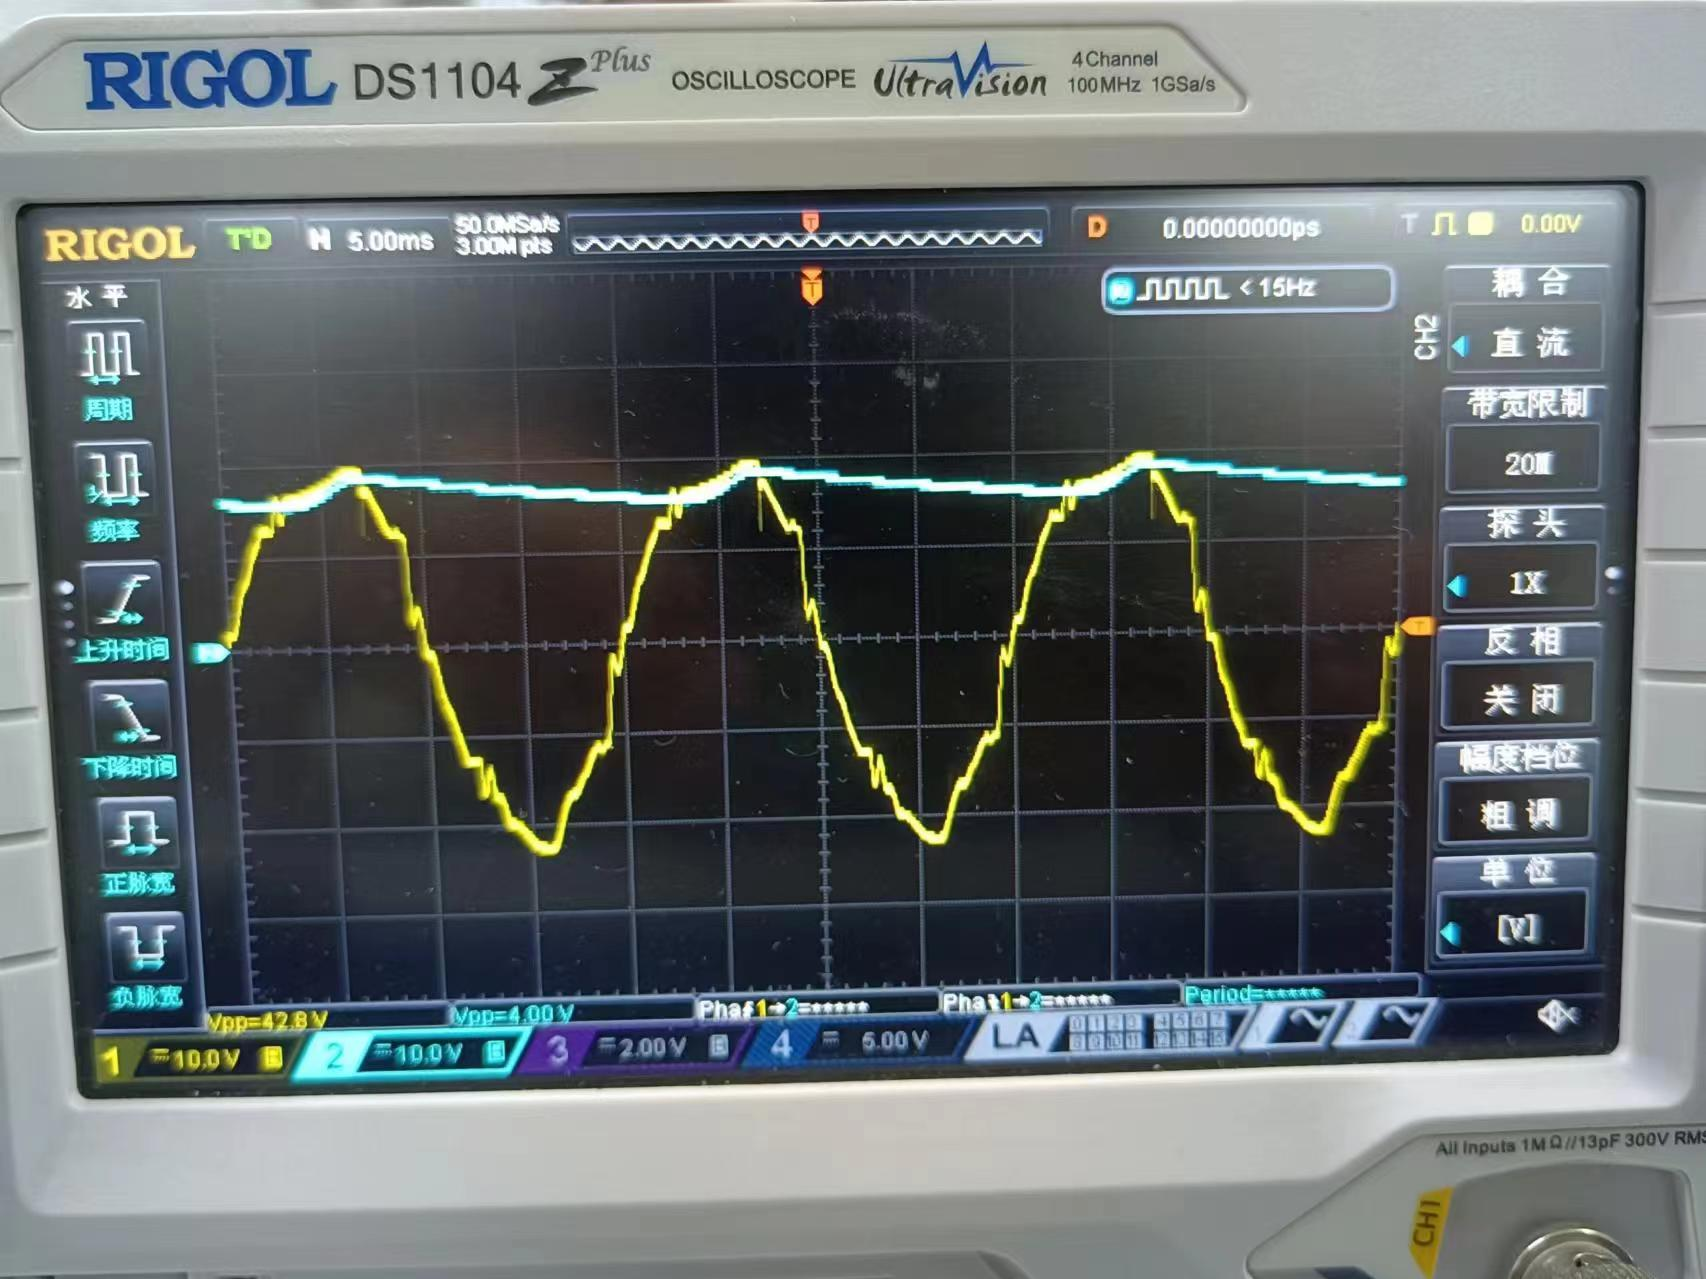
\includegraphics[width=0.4\linewidth]{滤波半波原始比较.jpg}
		\caption{纹波图像}
		\label{}
	\end{figure}

实验参数:$1200\Omega\quad 470\mu F$负载电阻增大。
\begin{figure}[{H}]
	\centering
	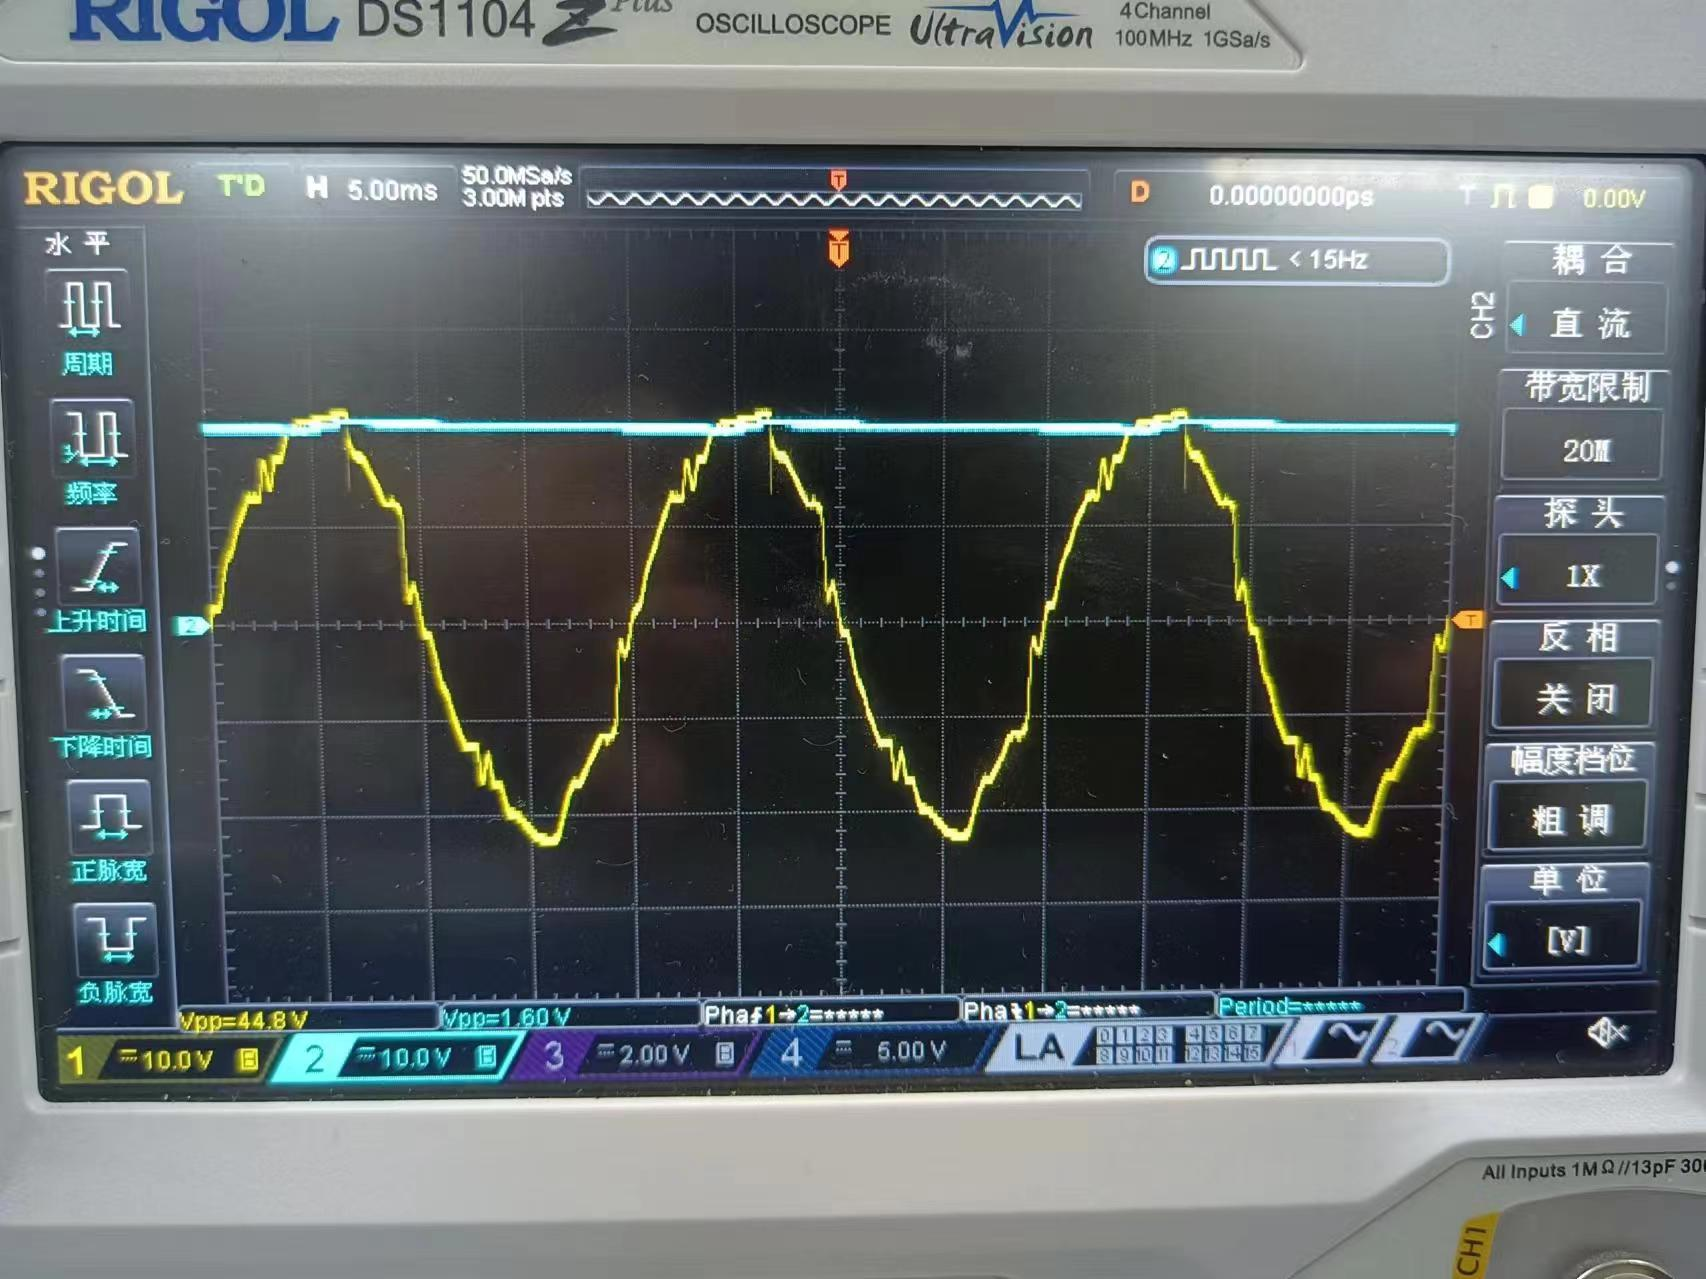
\includegraphics[width=0.3\linewidth]{滤波半波电阻增大.jpg}
	\caption{纹波图像}
	\label{}
\end{figure}
实验参数:$200\Omega\quad 47\mu F$滤波电容减小。
\begin{figure}[{H}]
	\centering
	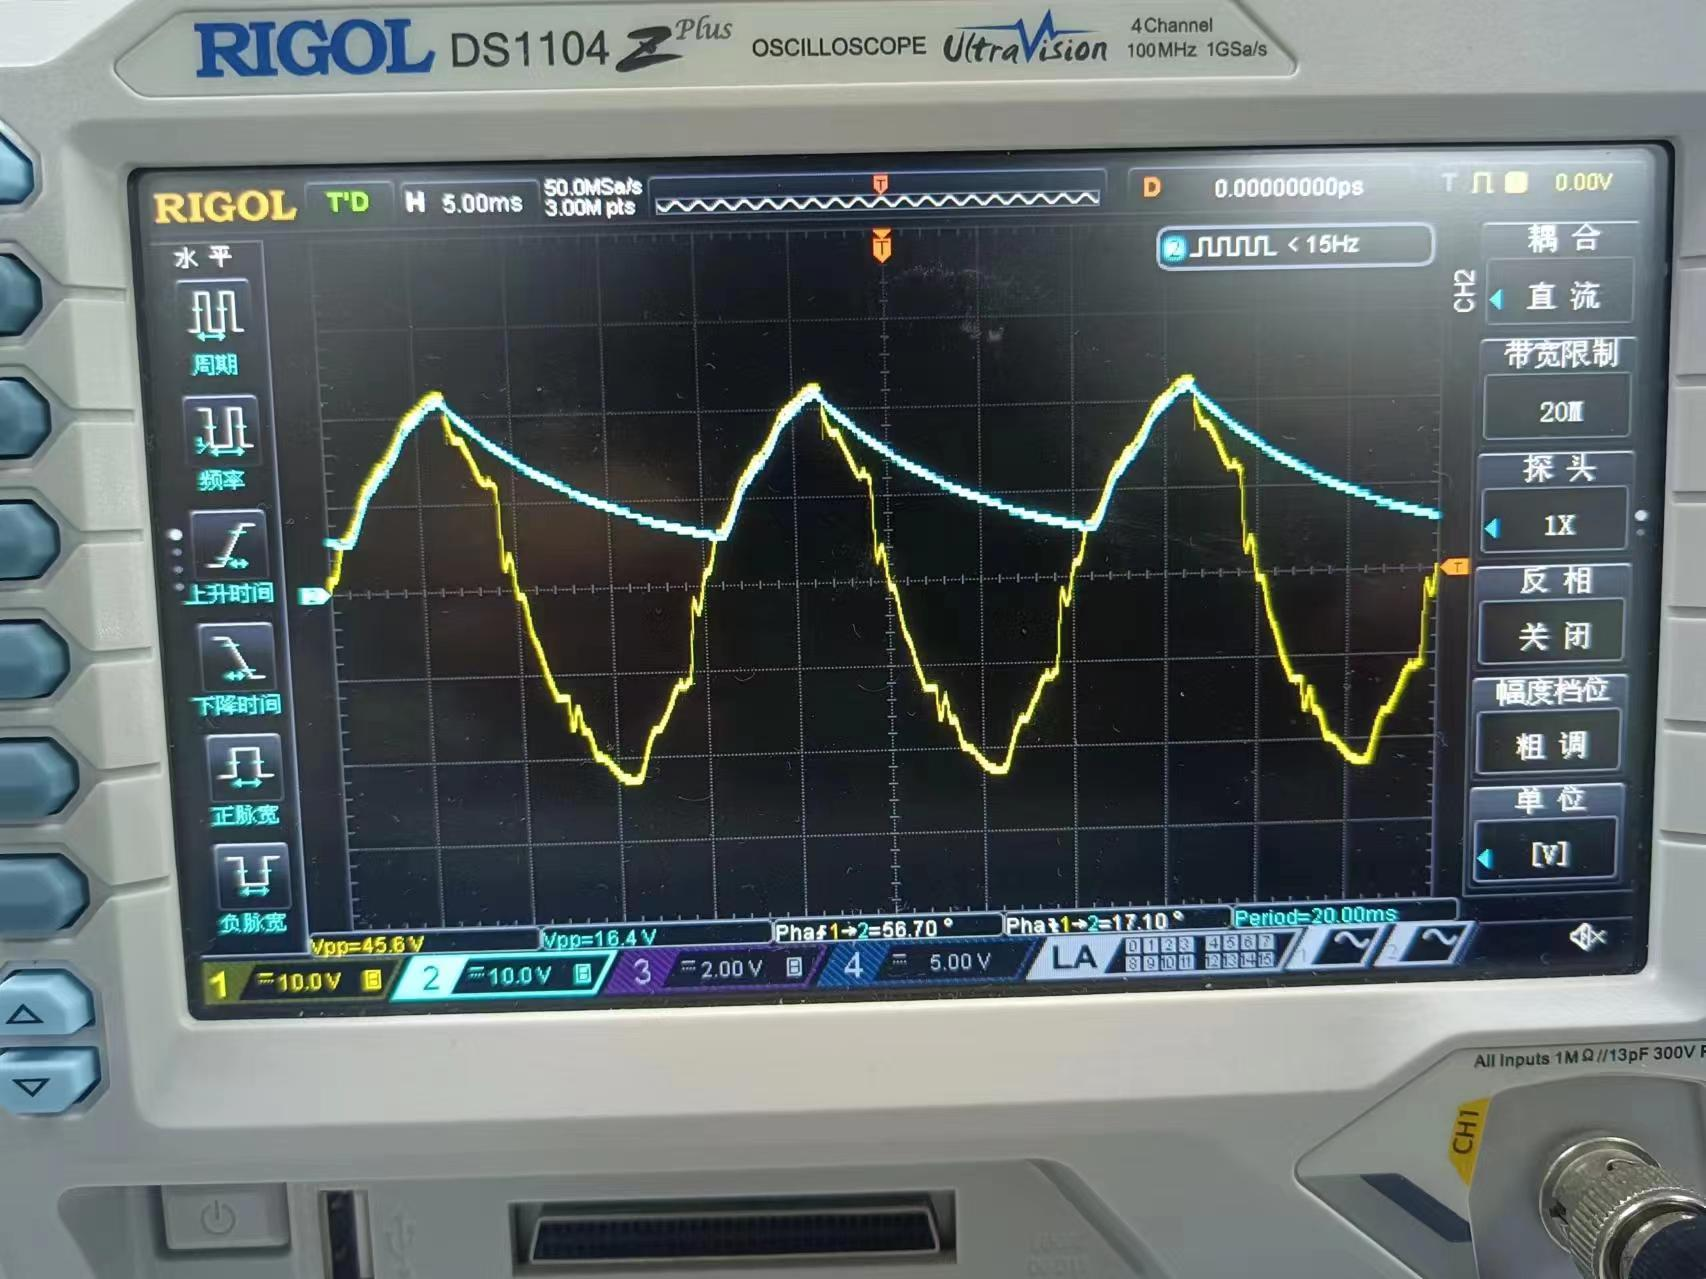
\includegraphics[width=0.4\linewidth]{滤波半波电容减小.jpg}
	\caption{纹波图像}
	\label{}
\end{figure}
\item 全波整流

	实验参数:$200\Omega\quad 470\mu F$
\begin{figure}[{H}]
	\centering
	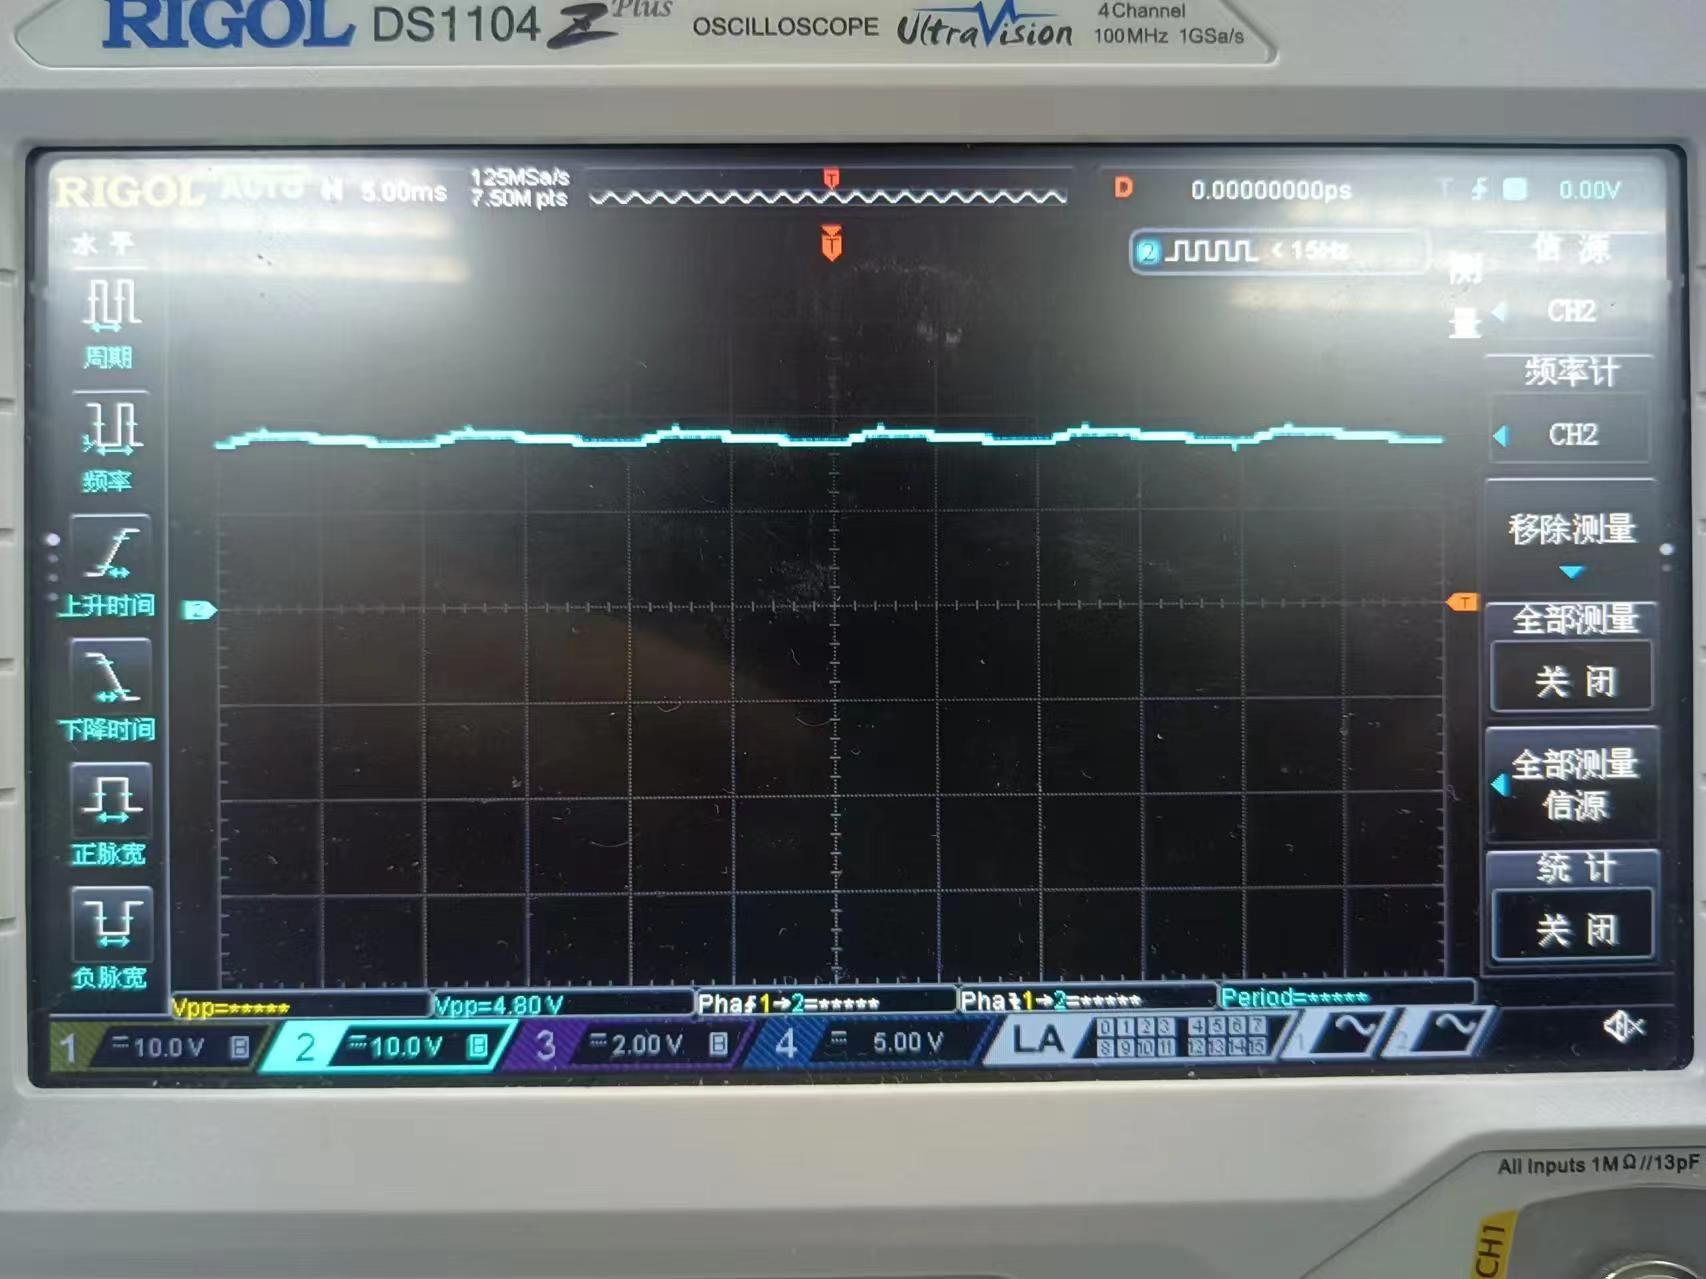
\includegraphics[width=0.4\linewidth]{滤波全波原始.jpg}
	\caption{纹波图像}
	\label{}
\end{figure}

实验参数:$1200\Omega\quad 470\mu F$负载电阻增大。
\begin{figure}[{H}]
	\centering
	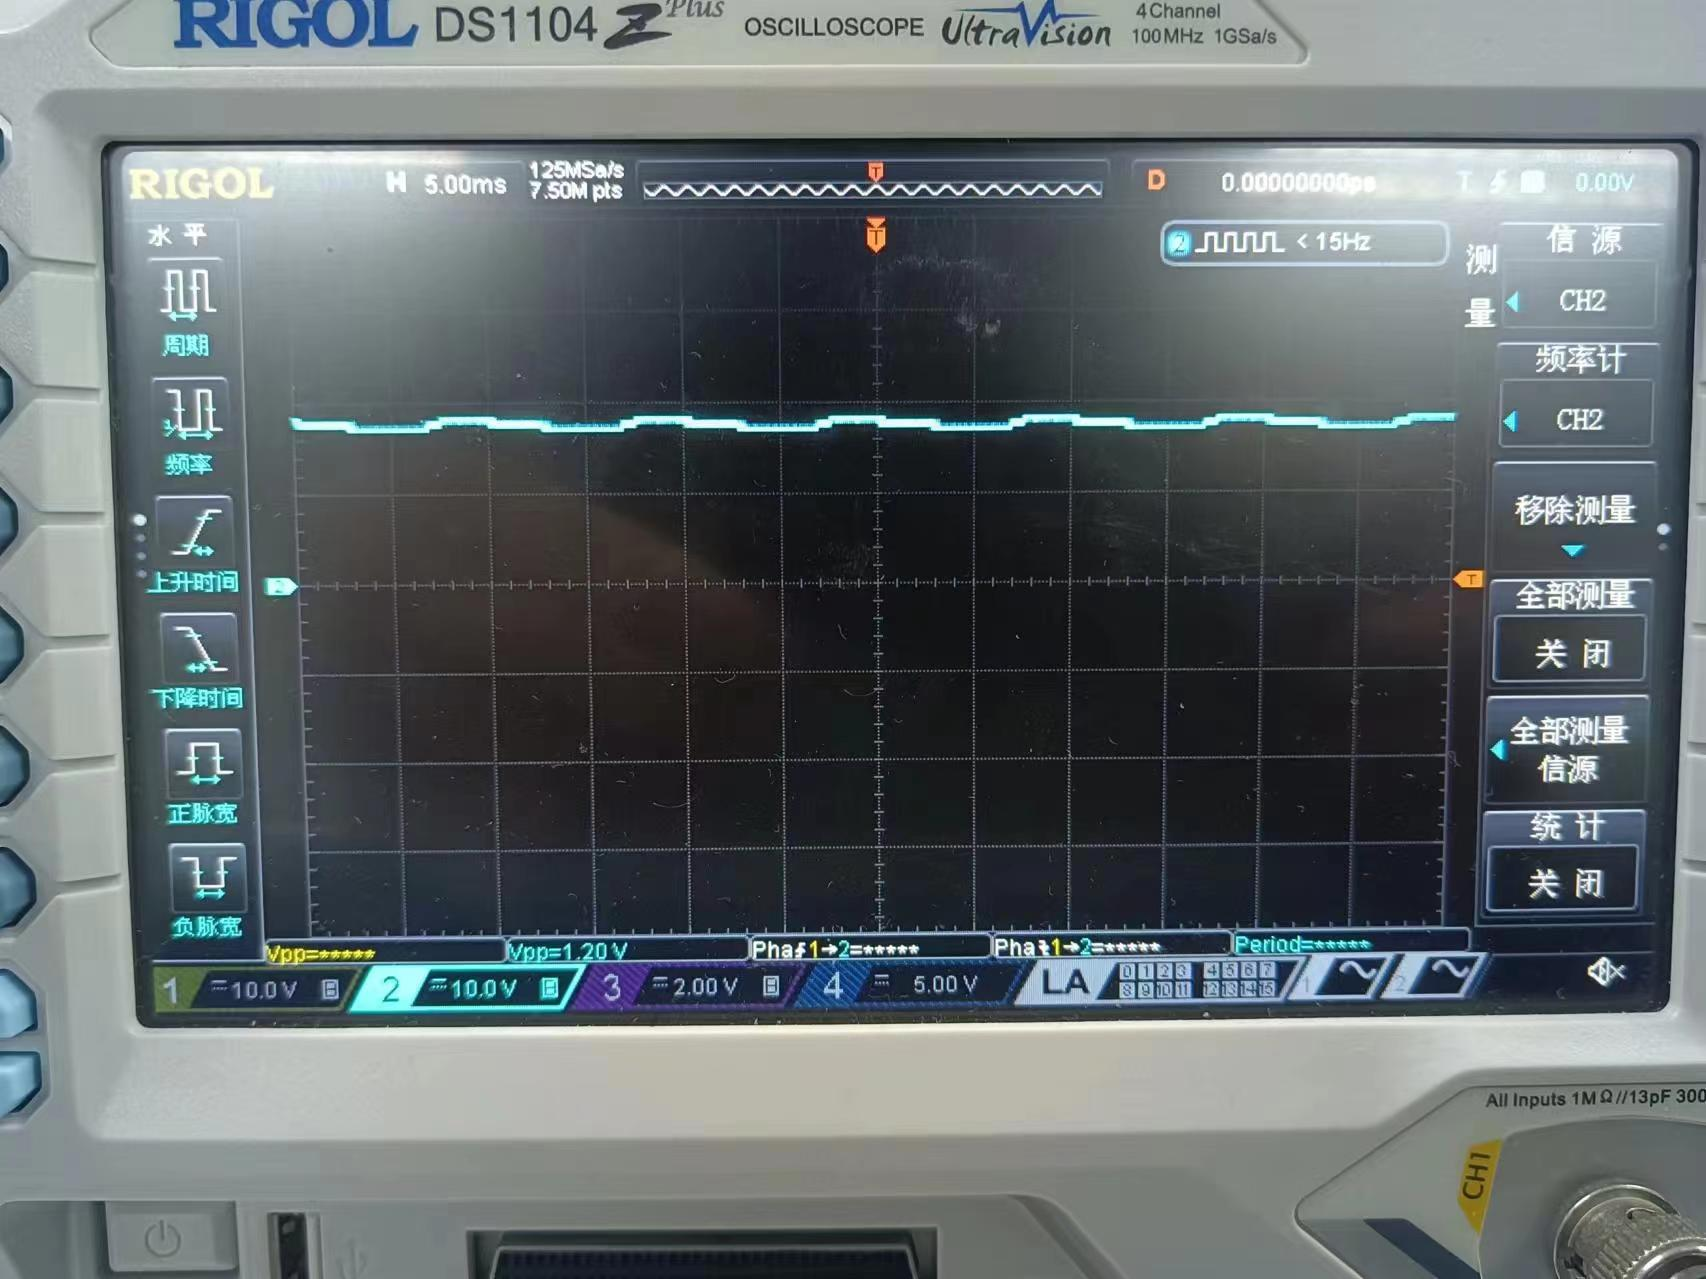
\includegraphics[width=0.4\linewidth]{滤波全波电阻增大.jpg}
	\caption{纹波图像}
	\label{}
\end{figure}
实验参数:$200\Omega\quad 47\mu F$滤波电容减小。
\begin{figure}[{H}]
	\centering
	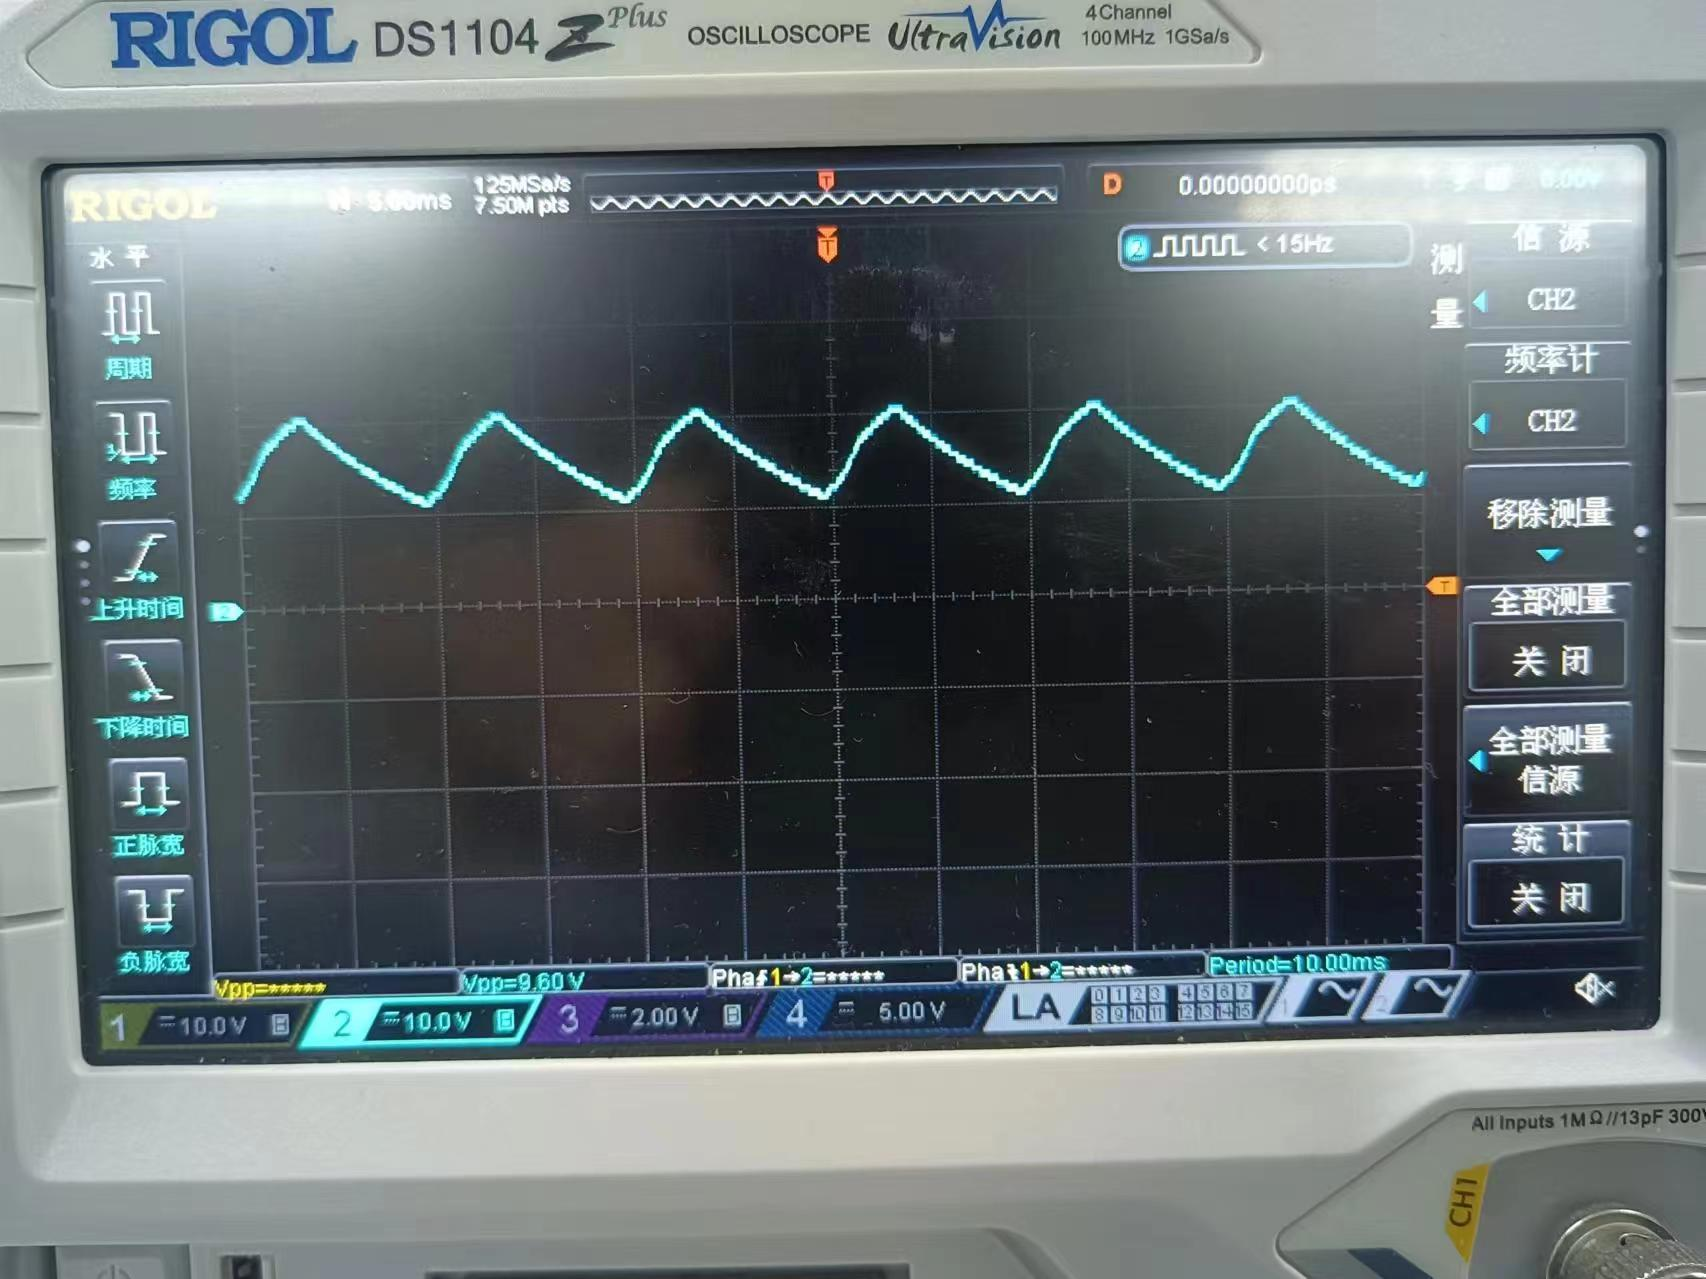
\includegraphics[width=0.3\linewidth]{滤波全波电容减小.jpg}
	\caption{纹波图像}
	\label{}
\end{figure}
 

\end{enumerate}

	\subsubsection{在桥式整流滤波电路中,搭建稳压管并联稳压电路}

调整负载大小(120ohm,240ohm,360ohm),观测并记录稳压电路的稳压效果;
\begin{figure}[H]
	\begin{minipage}[b]{0.3\linewidth}
	  \centering
	  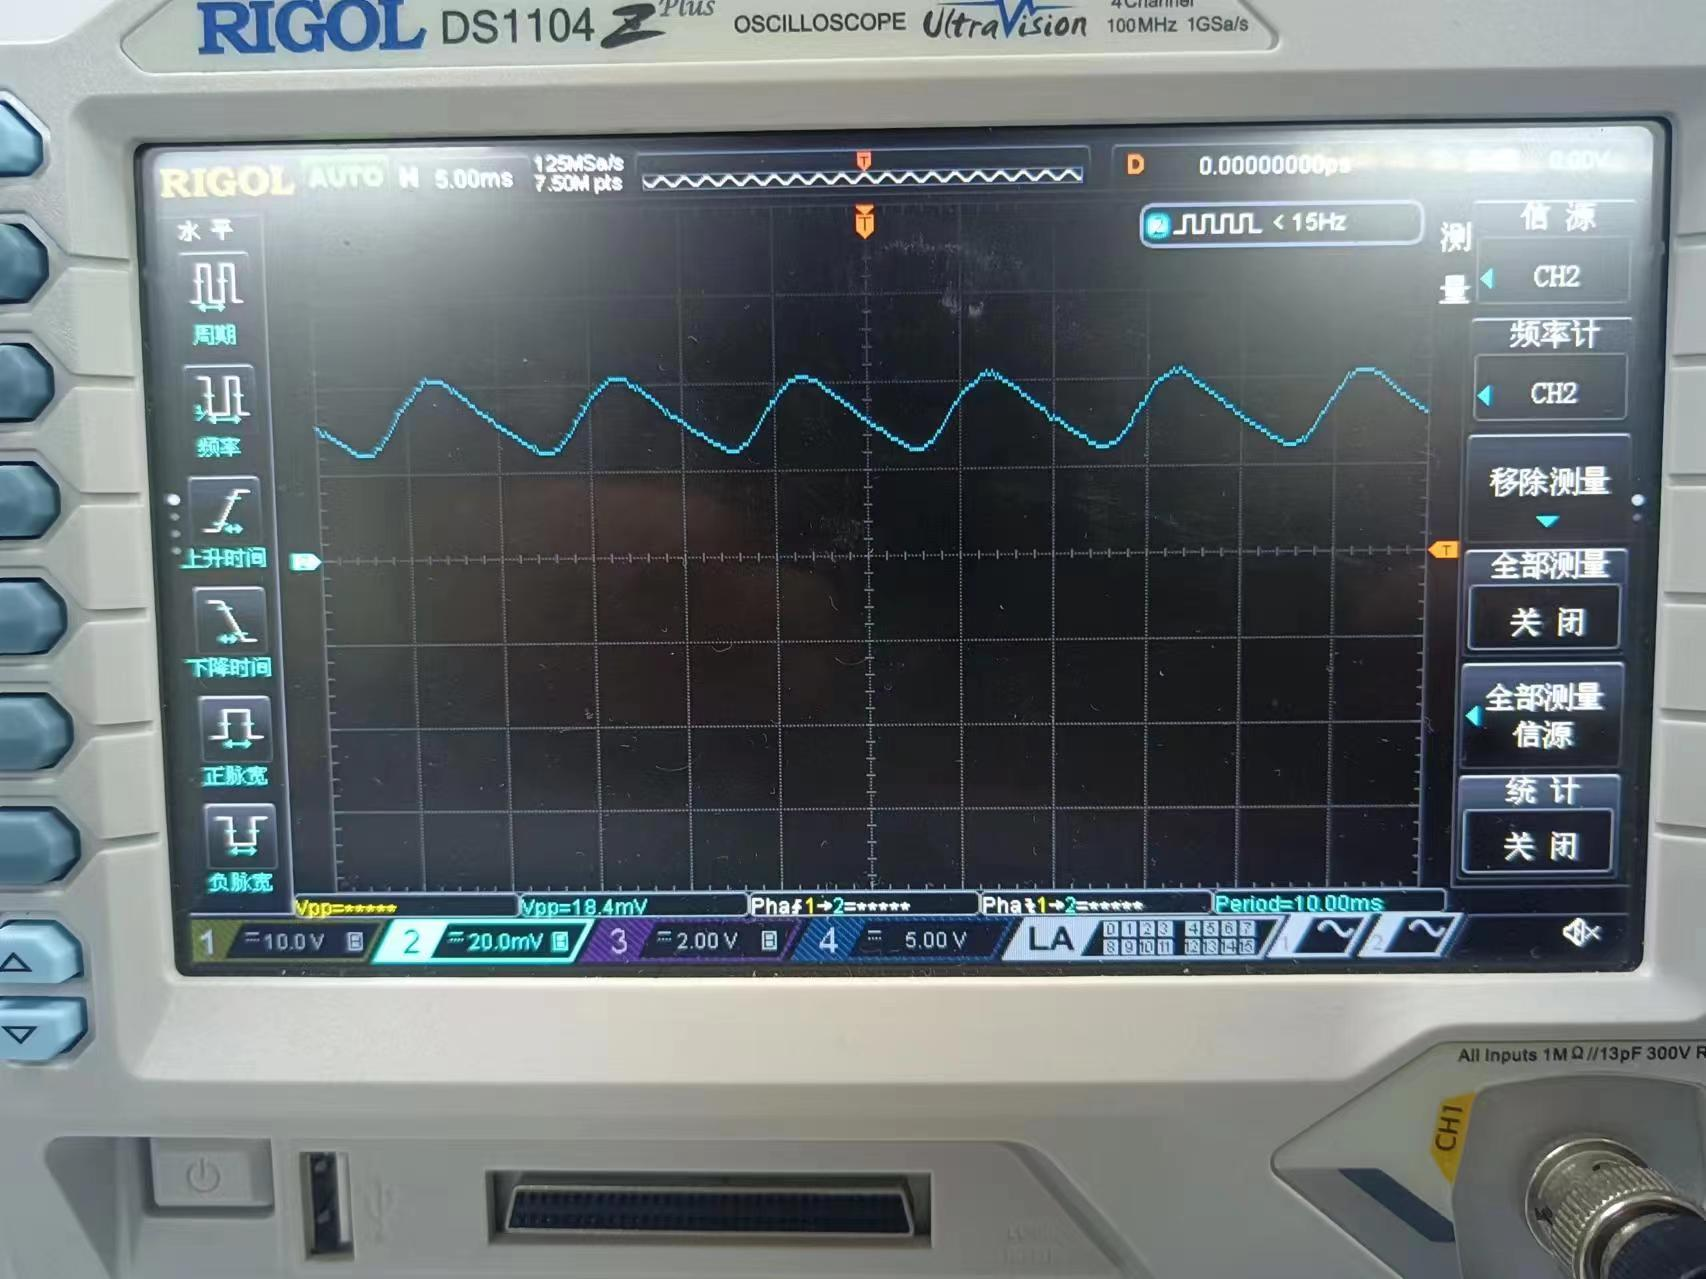
\includegraphics[width=\linewidth]{41.jpg}
	
	\end{minipage}
	\hfill
	\begin{minipage}[b]{0.3\linewidth}
	  \centering
	  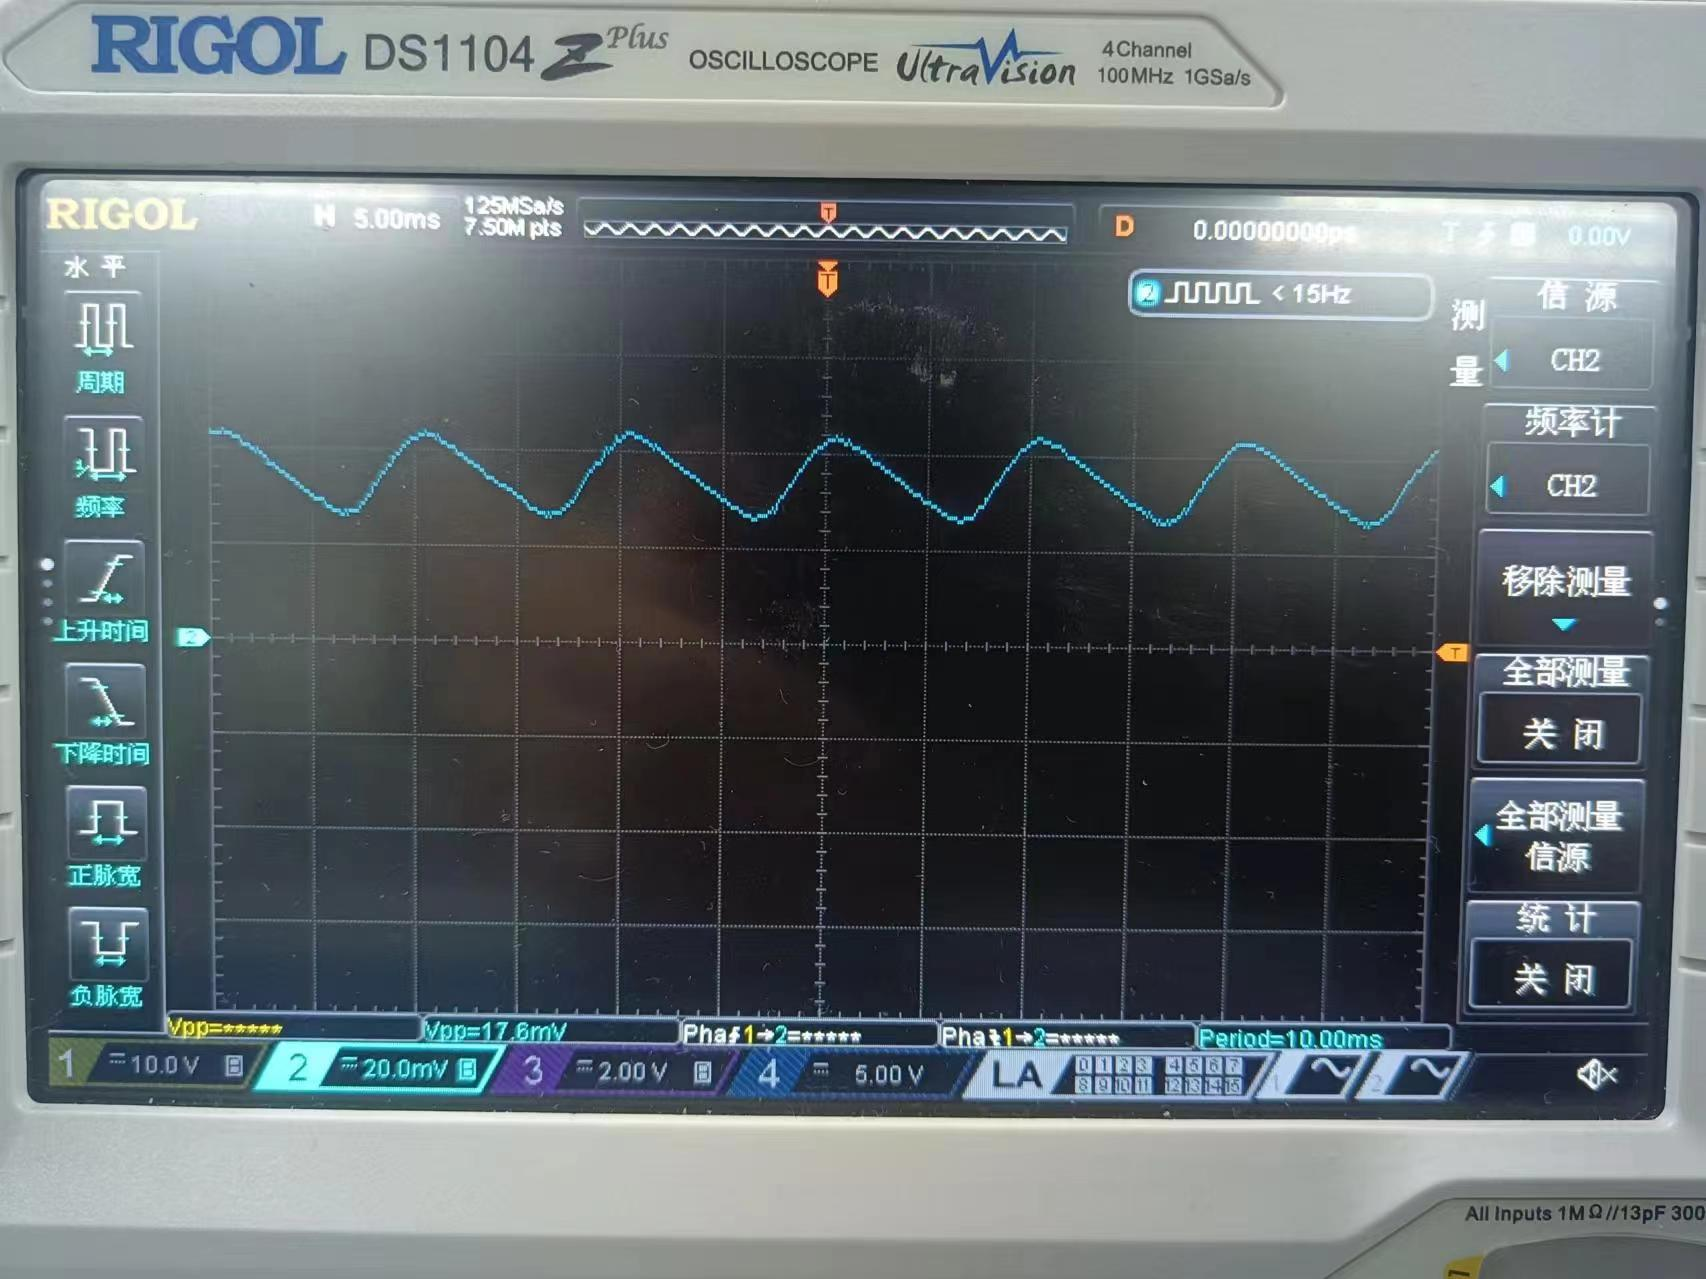
\includegraphics[width=\linewidth]{42.jpg}
	
	\end{minipage}
	\hfill
	\begin{minipage}[b]{0.3\linewidth}
	  \centering
	  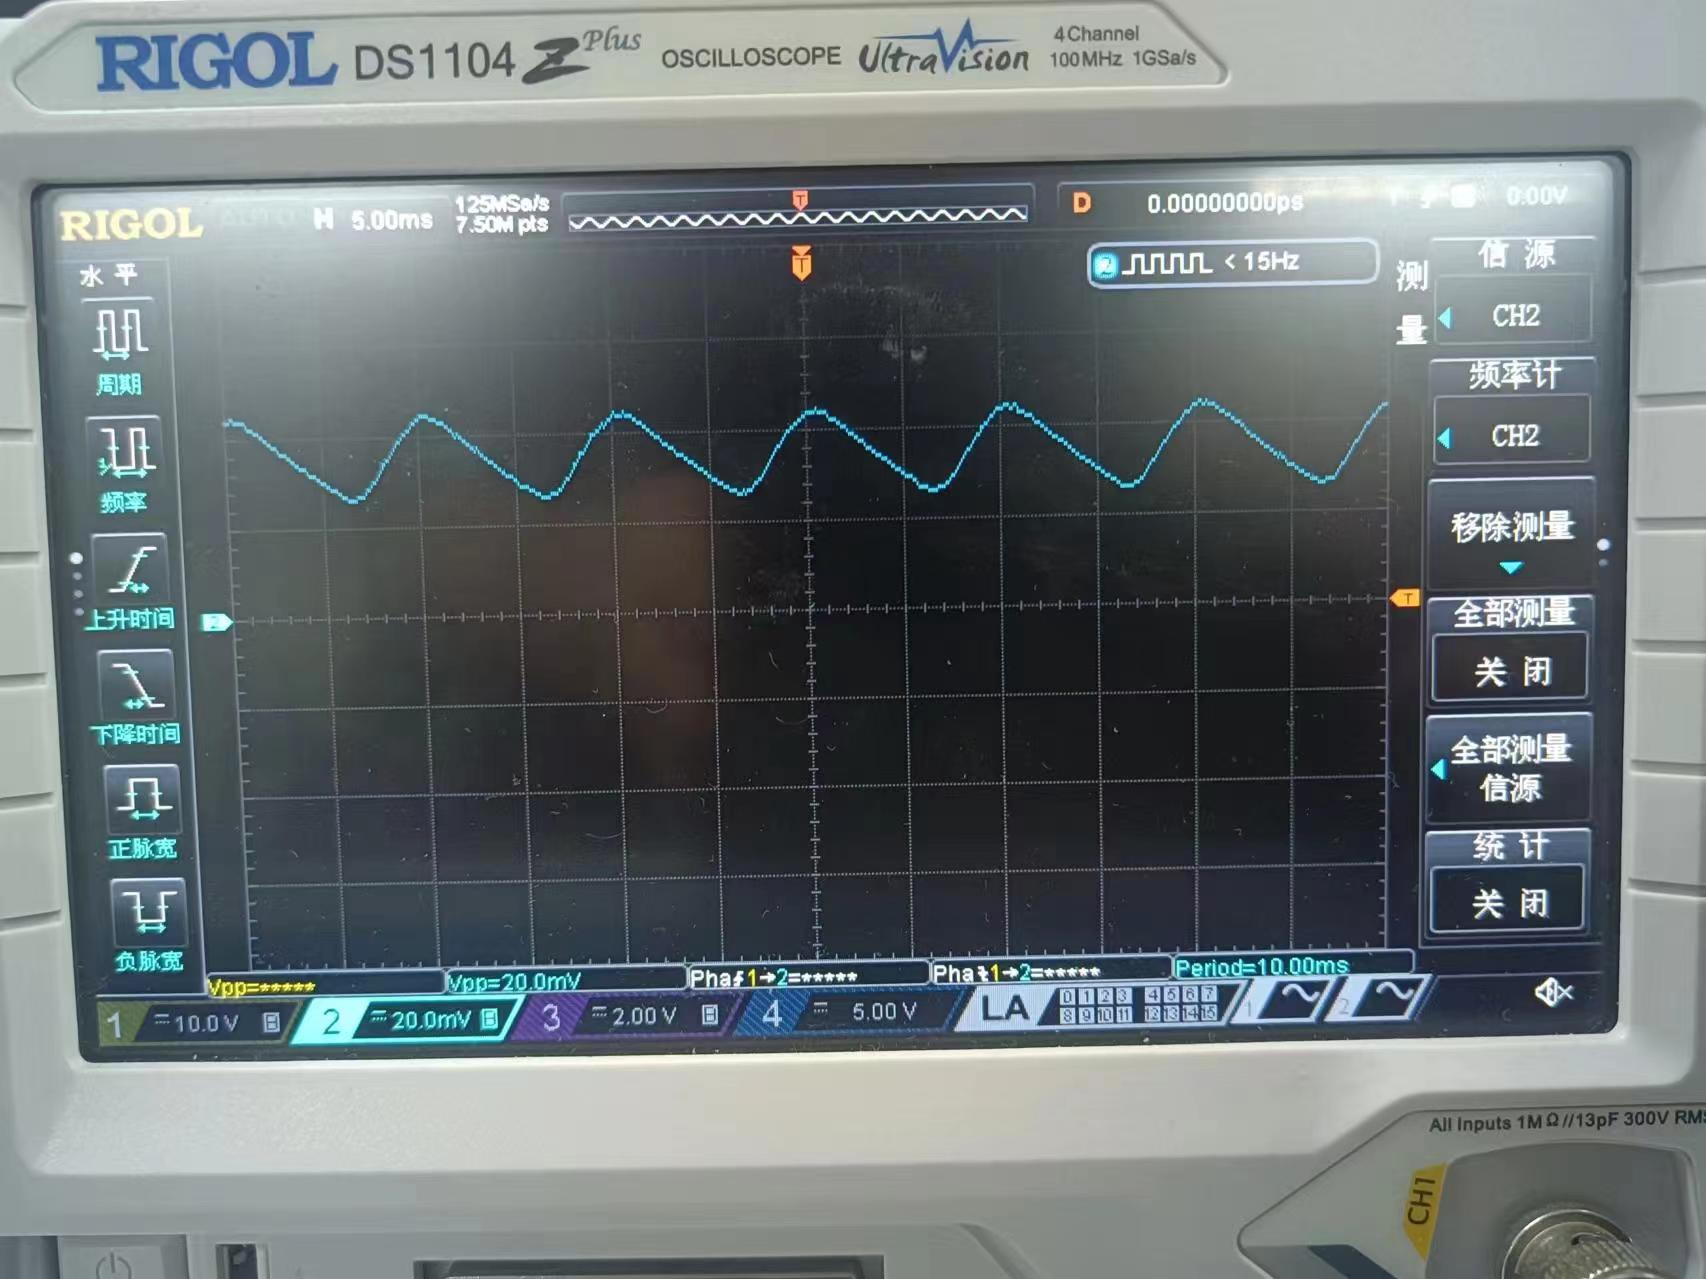
\includegraphics[width=\linewidth]{43.jpg}
	  
	\end{minipage}
\end{figure}
\begin{table}[H]
    \centering
    \caption{实验数据}
    \begin{tabular}{|c|c|c|c|c|c|c|}
        \hline
        负载 (Ω) & Ii (mA) & Ui (V) & Pi (W) & Io (mA) & Uo (mV) & Po (W) \\
        \hline
        120 & 14.67 & 2.93 & 0.0430 & 164.025 & 33.325 & 5.466 \\
        \hline
        240 & 14.85 & 2.95 & 0.0438 & 145.952 & 35.162 & 5.132 \\
        \hline
        360 & 14.88 & 2.97 & 0.0442 & 97.422 & 35.529 & 3.461 \\
        \hline
    \end{tabular}
\end{table}

\subsubsection{在桥式整流滤波电路中,搭建集成三端稳压器稳压电路}
\begin{figure}[H]
	\begin{minipage}[b]{0.3\linewidth}
	  \centering
	  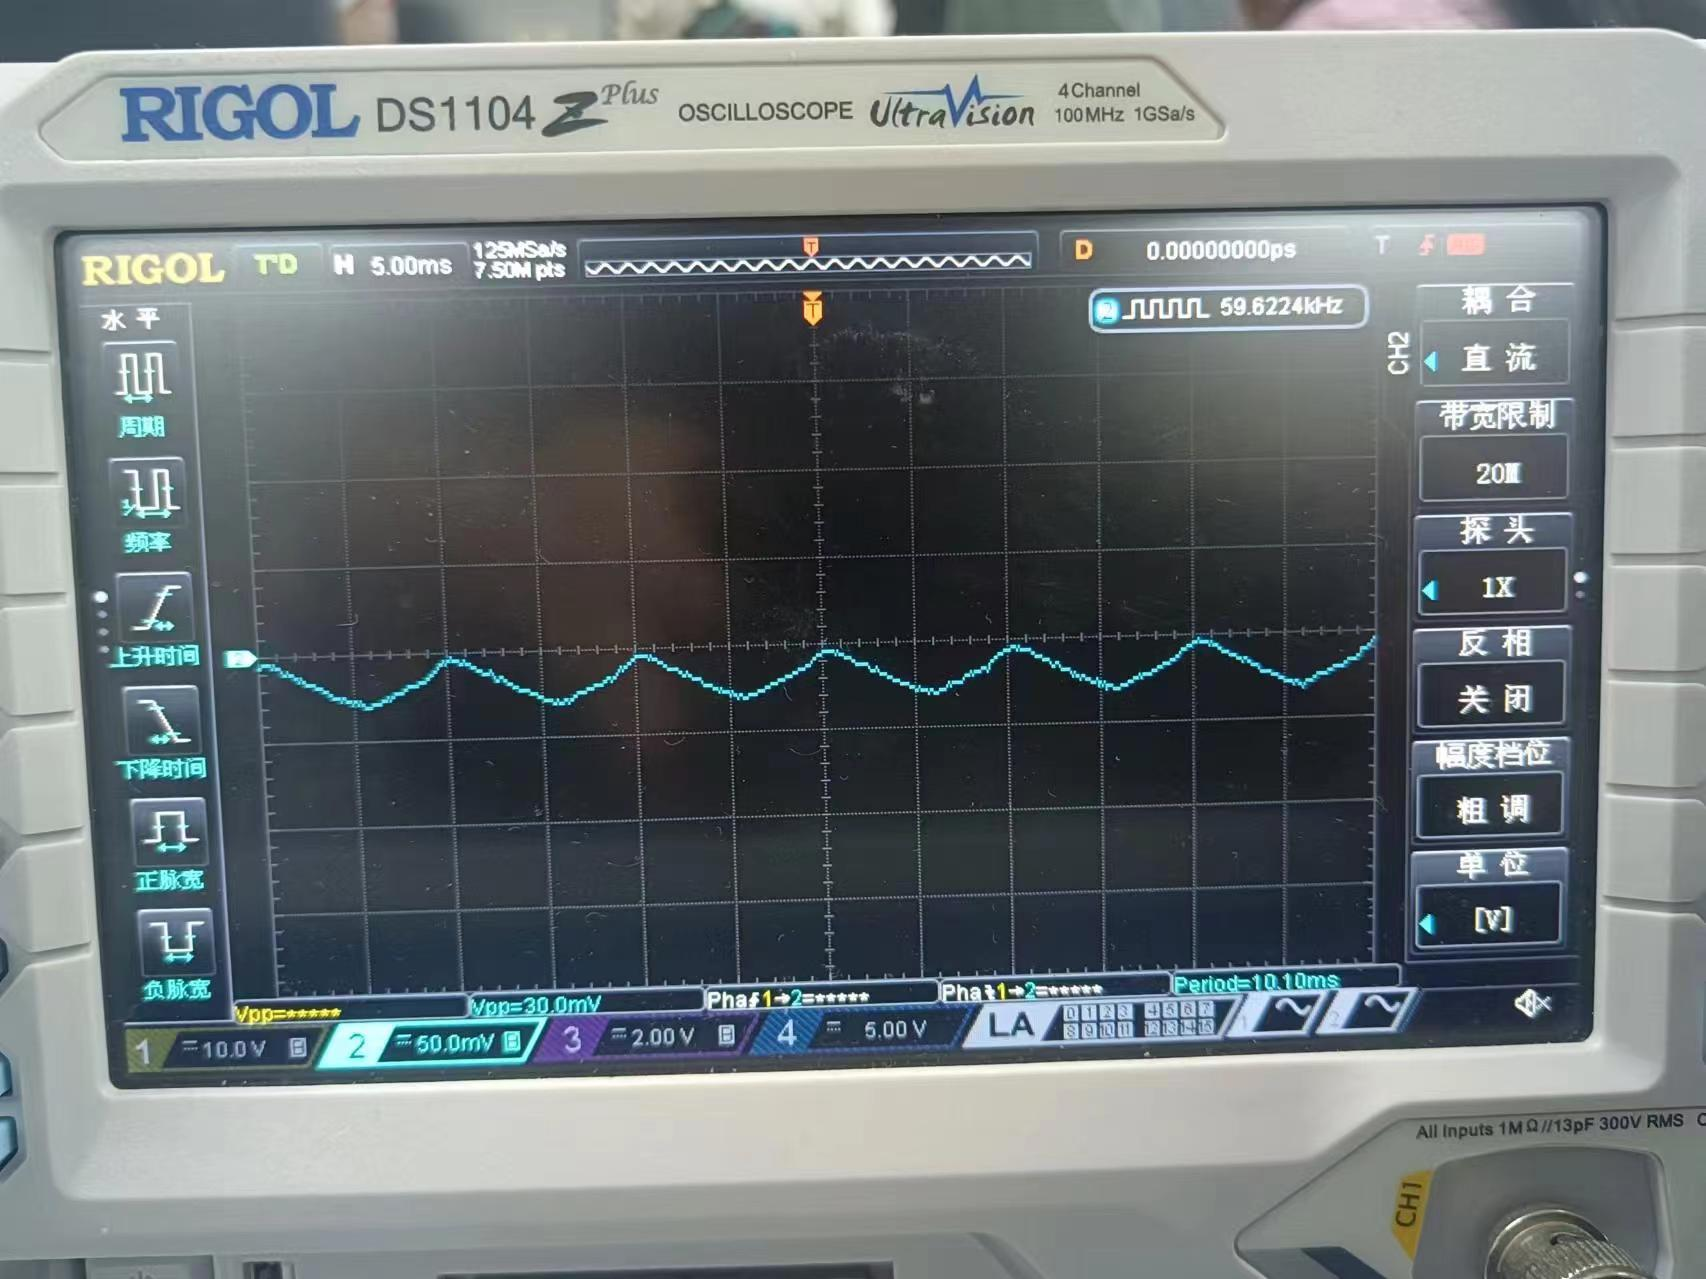
\includegraphics[width=\linewidth]{51.jpg}
	  \caption{}
	\end{minipage}
	\hfill
	\begin{minipage}[b]{0.3\linewidth}
	  \centering
	  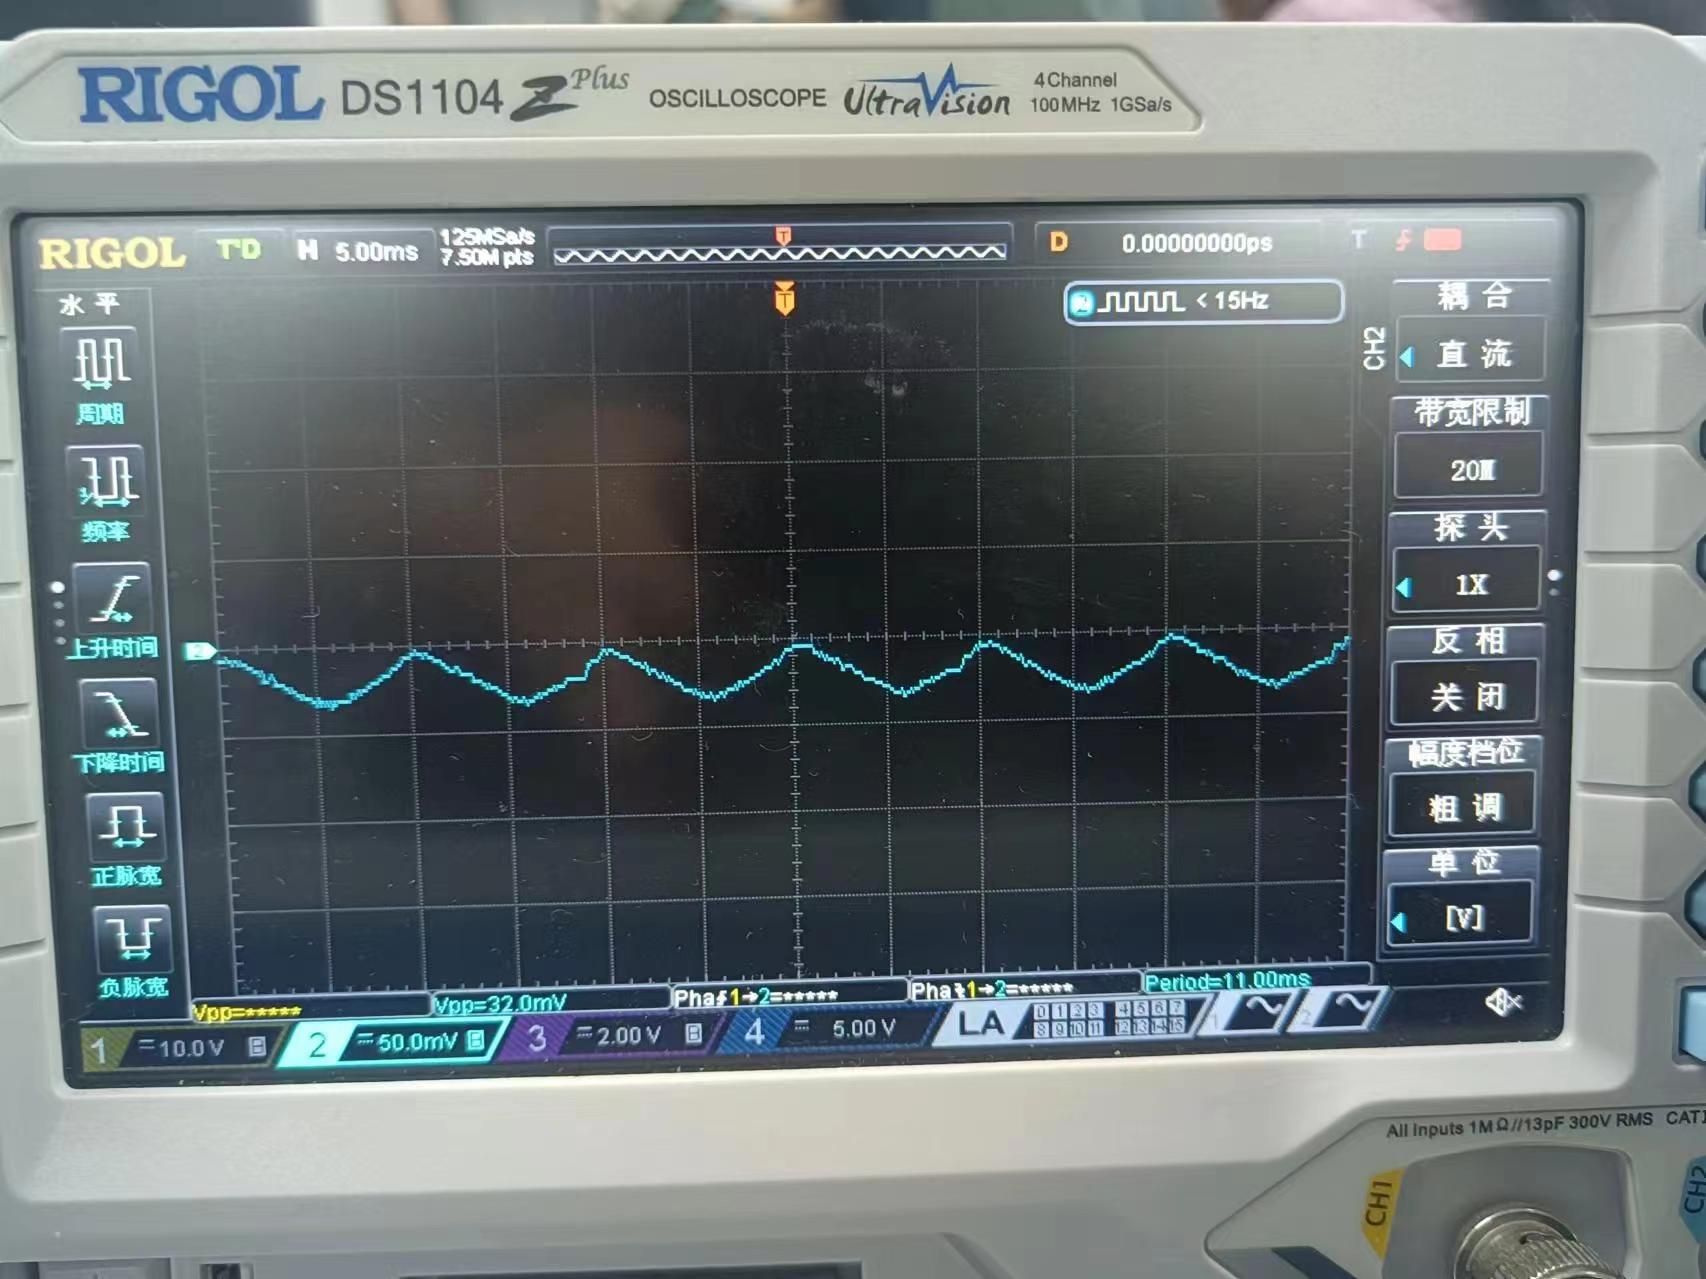
\includegraphics[width=\linewidth]{52.jpg}
	  \caption{}
	\end{minipage}
	\hfill
	\begin{minipage}[b]{0.3\linewidth}
	  \centering
	  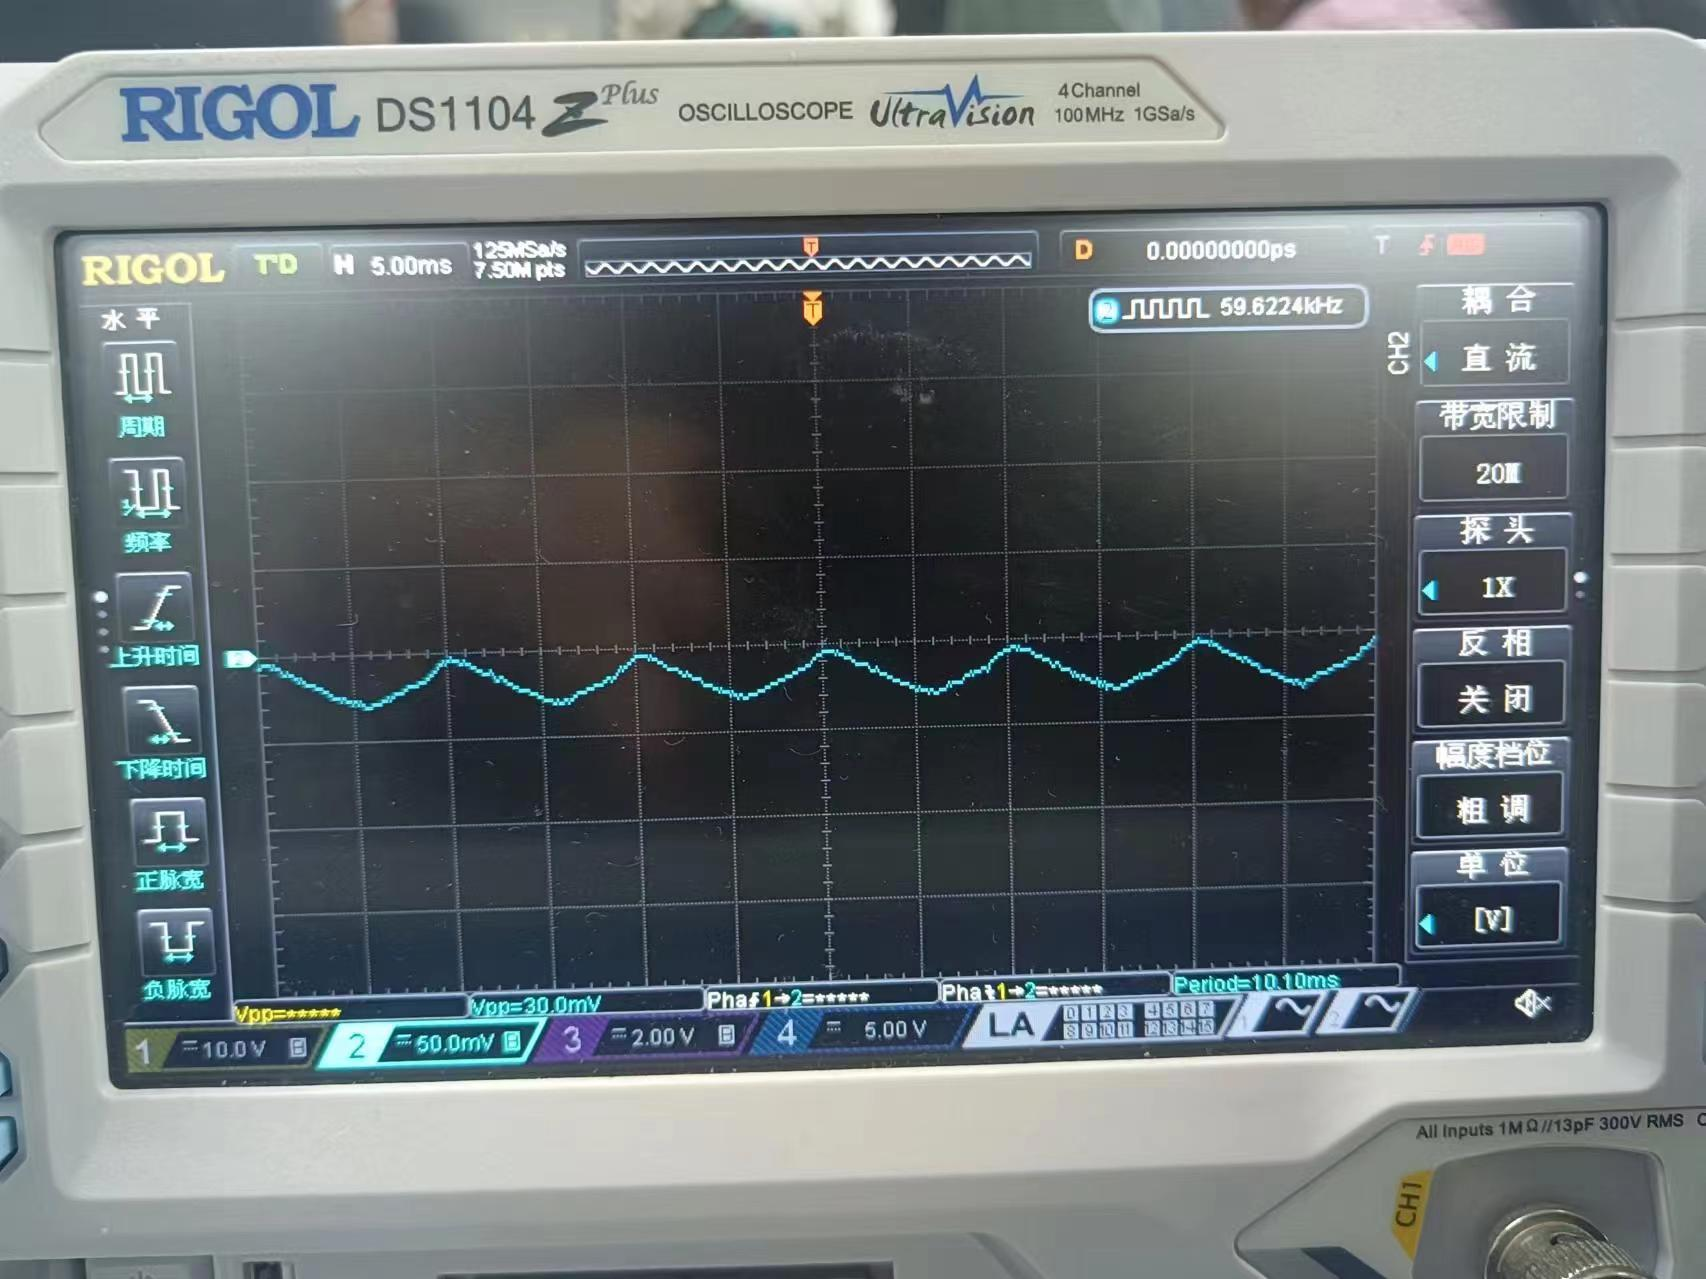
\includegraphics[width=\linewidth]{53.jpg}
	  \caption{}
	\end{minipage}
\end{figure}
\begin{table}[H]
    \centering
    \caption{实验数据}
    \begin{tabular}{|c|c|c|c|c|c|c|}
        \hline
        负载 (Ω) & Ii (mA) & Ui (V) & Pi (W) & Io (mA) & Uo (V) & Po (W) \\
        \hline
        120 & 129.13 & 15.17 & 1.959 & 110.3 & 13.27 & 1.464 \\
        \hline
        240 & 138.56 & 14.25 & 1.974 & 59.3 & 14.29 & 0.847 \\
        \hline
        360 & 145.67 & 14.18 & 2.066 & 40.2 & 14.56 & 0.585 \\
        \hline
    \end{tabular}
\end{table}
	
	% 问题记录
	\subsection{实验过程遇到问题及解决办法}
	\begin{enumerate}
		\item 实验中的测量方式存在一定的实验问题,出现了相关的很严重的实验误差。
		\item 实验中的电路连接和判断所测数据相对较难,需要经过一些讨论。
	\end{enumerate}
	% ---
	
	
	
	% 分析与讨论	
	\clearpage
	
	% 顶栏
	\begin{table}
		\renewcommand\arraystretch{1.7}
		\begin{tabularx}{\textwidth}{|X|X|X|X|}
			\hline
			专业:& 物理学 &年级:& 2022级\\
			\hline
			姓名: &黄罗琳、王显  & 学号:&22344001、22344002 \\
			\hline
			日期:& 2024/6/12 & 评分: &\\
			\hline
		\end{tabularx}
	\end{table}
	% ---
	
	% 小标题
	\section{ET13整流滤波与稳压电路 \quad\heiti 分析与讨论}
	% ---
	
	% 数据处理
	\subsection{实验数据分析}
	\begin{enumerate}
 \item 搭建半波整流电路,用示波器观测和记录输出波形;
交流电经过半波整流电路后,一个周期内一半时间有波形显示,一半时间为0。






\item 搭建桥式整流电路, 用示波器观测和记录输出波形;
交流电经过桥式整流电路后,一个周期内没有输出为零,存在周期波形。







\item 加入滤波电容
 在刚刚全波桥式整流电路的基础上,加入滤波电容后,得到的结果如图12-17所示:

半波整流+电容滤波:负载电阻增大,纹波减小;滤波电容增大,纹波减小。
桥式整流+电容滤波:负载电阻增大,纹波没有明显;滤波电容增大,纹波减小。

 \item 在桥式整流滤波电路中,搭建稳压管并联稳压电路,调整负载大小,观测并记录稳压电路的稳压效果;
观察实验图像数据可知,随着负载增大,纹波数据小幅度减小,可以认为稳压效果更好了。




\item 在桥式整流滤波电路中,搭建集成三端稳压器稳压电路 ,调整负载大小,观测并记录稳压电路的稳压效果;
观察实验图像数据可知,随着负载增大,纹波数据小幅度减小,可以认为稳压效果更好\textbf{(存疑)}。
\item 比较实验45电路中稳压电路的输入输出效率;

	\begin{table}[H]
		\centering
		\caption{实验4和实验5的数据及计算结果}
		\begin{tabular}{|c|c|c|}
			\hline
			实验 & 负载 (Ω) & $\frac{Po}{Pi} \times 100\%$ \\
			\hline
			实验4 & 120 & 12.71\% \\
			\hline
			实验4 & 240 & 11.72\% \\
			\hline
			实验4 & 360 & 7.83\% \\
			\hline
			实验5 & 120 & 74.73\% \\
			\hline
			实验5 & 240 & 42.91\% \\
			\hline
			实验5 & 360 & 28.32\% \\
			\hline
		\end{tabular}
	\end{table}
	明显看出,使用集成三端稳压器的效率明显比稳压管电路高,并且电路负载越小,电路效率越高。
\end{enumerate}

	\subsection{实验后思考题}
	
	%思考题1
	\begin{question}
		比较半波整流与桥式整流的特点
	\end{question}
	半波整流只能获取一半的正信号,而桥式整流能够获得完整的同向信号。

	半波整流器利用二极管的单向导电特性,只在交流电的正半周期时导通,将正半周期的电流传输给负载,而在负半周期时则截止,电流被阻断。这样,负载上只会出现正半周期的电流,而负半周期的电流则被抑制。
	
	而桥式整流器通过四个二极管组成桥式电路,能够在交流电的正、负半周期都将电流整流为同一方向的直流电。当输入交流电为正半周期时,对角的两个二极管导通,电流通过负载;当输入交流电为负半周期时,另对角的两个二极管导通,体现完整的信号。
	% 思考题2
	\begin{question}
		滤波电容C的作用。
	\end{question}
	电容在电路中起到滤波的作用,主要通过其充放电特性来平滑电压波形,从而滤除变化幅度较大且频率较快的信号。在整流电路中,整流后的直流电压通常包含脉动成分,这些脉动会导致电压不稳定,影响后续电路的正常工作。为了解决这一问题,常常在整流电路后面添加一个电容作为滤波器。

当整流后的脉动电压加到滤波电容上时,电容开始充电,电压逐渐上升到脉动电压的峰值。在电源电压下降期间,电容由于其储能特性不会立即放电,而是缓慢放电。这种缓慢放电的特性使得电容能够在电源电压下降时仍然提供电流,维持输出电压相对稳定,减小电压的脉动幅度。

具体来说,当电源电压高于电容电压时,电容充电;当电源电压低于电容电压时,电容放电。由于电容的放电过程较为缓慢,它可以在电源电压下降的过程中释放储存的电能,抵消部分电压波动,从而在负载两端提供较为平滑的直流电压。

通过这种方式,电容滤波器能够有效滤除高频噪声和脉动成分,使输出电压更加平滑和稳定。不同容量的电容对不同频率的噪声和脉动具有不同的滤波效果,通常容量越大,滤波效果越好,可以滤除更低频率的波动。因此,在实际电路设计中,根据需要选择合适容量的电容,以达到最佳的滤波效果。

	% 思考题3
	\begin{question}
		稳压二极管稳压作用。
	\end{question}
	稳压二极管的最主要作用是电压稳压。在电源电路中,由于负载变化或电源波动,电压可能会出现不稳定的情况。稳压二极管通过其在反向击穿区域的稳定电压特性,可以提供一个恒定的输出电压,从而保证后续电路的稳定运行。无论输入电压如何变化,只要输入电压高于齐纳电压,稳压二极管就能将输出电压稳定在其击穿电压值附近。
	% ---
	
	
	% 结语部分
	\clearpage
	
	% 小标题
	\section{ET13整流滤波与稳压电路\quad\heiti 结语}
	% ---
	
	% 总结、杂谈与致谢
	\subsection{实验心得和体会、意见建议等}
	\begin{enumerate}
		\item 实验总体难度在于得到一个正确的实验数据,某些时候,尽管我们测出了一组数据,但是我们无法保证它的正确性,这种不自信根本在于电路仪器的测量精度、作用效果的质疑
		\item \textbf{本实验报告采用LATEX编辑,实验分工为黄罗琳同学负责记录数据、编辑报告、数据分析,王显同学负责实验操作、数据分析。}
	\end{enumerate}
	% ---
	

	% 附件
	\subsection{附件}
	\begin{figure}[{H}]
		\centering
		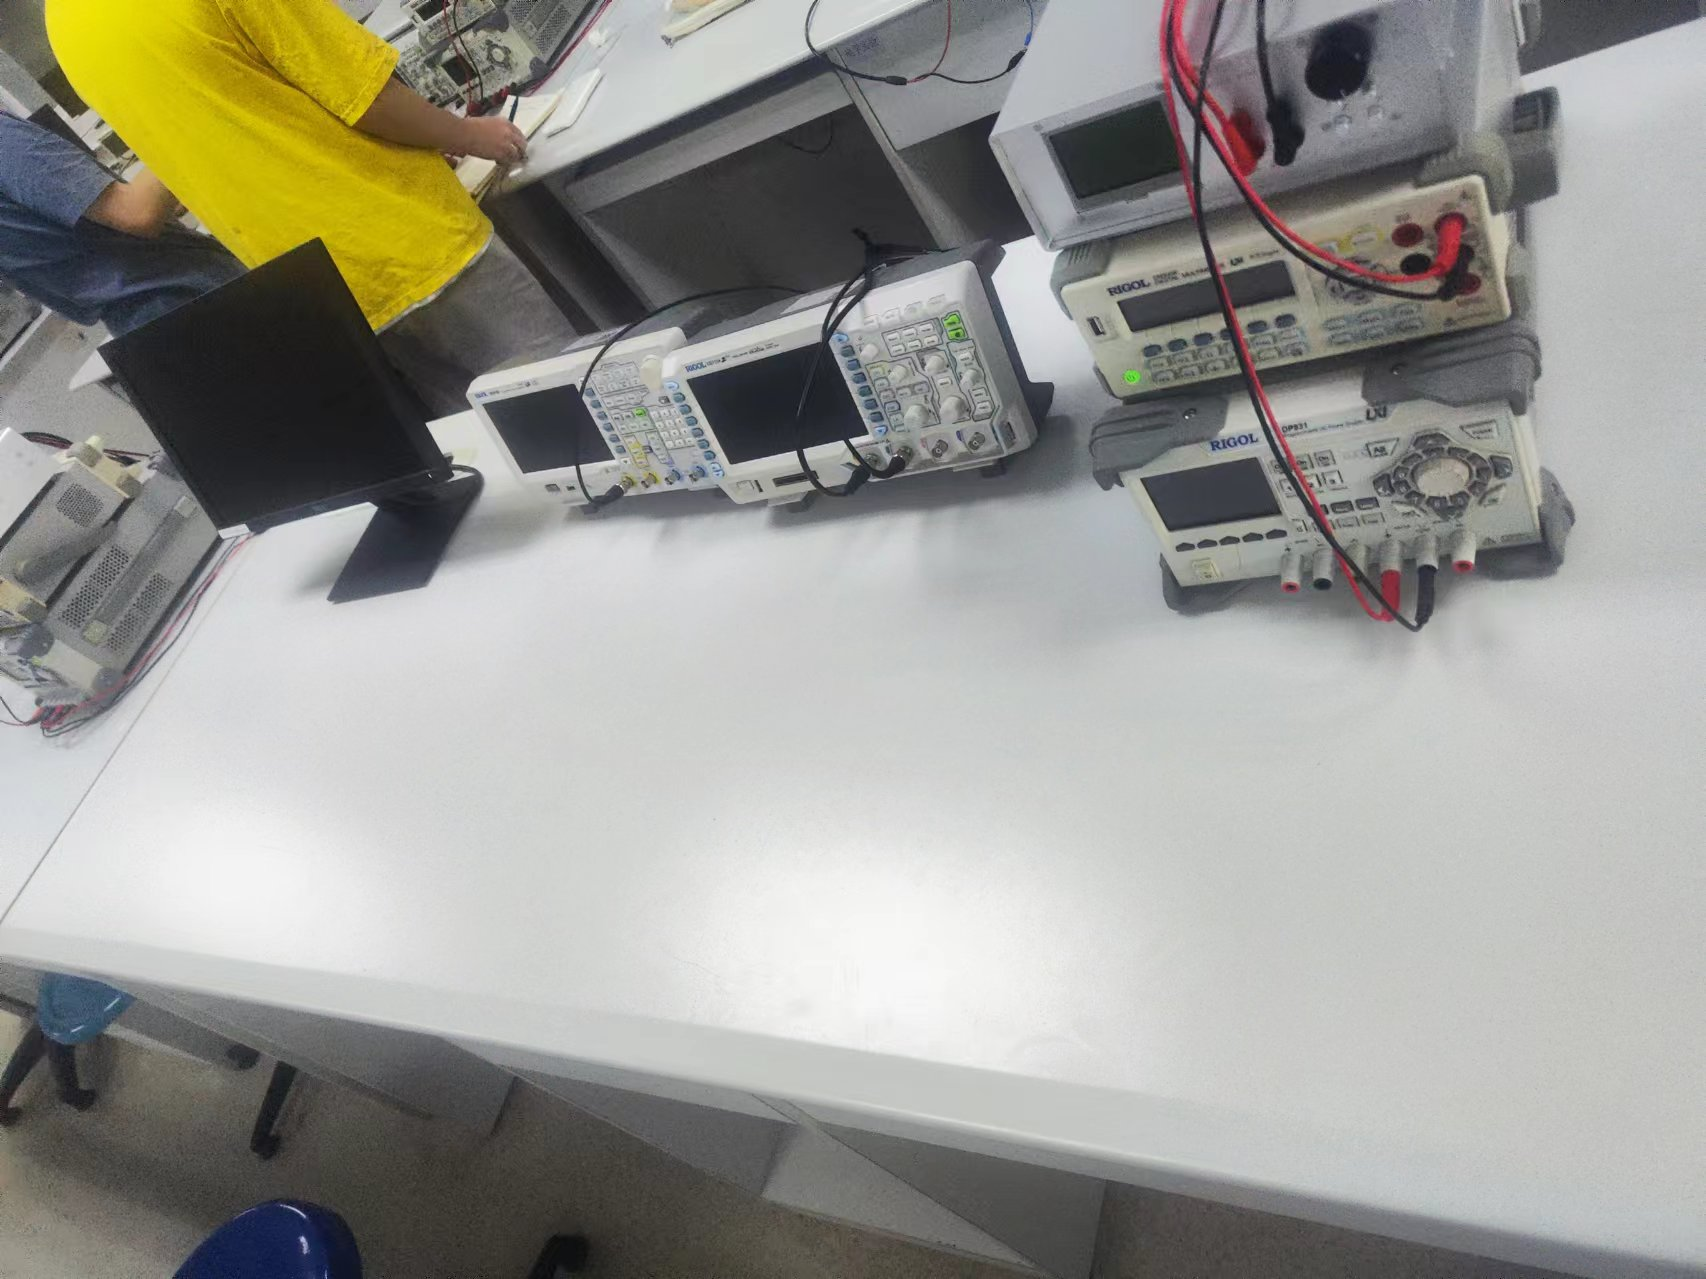
\includegraphics[width=0.4\linewidth]{桌面.jpg}
		\caption{桌面}
		\label{}
	\end{figure}
	\begin{figure}[{H}]
		\centering
		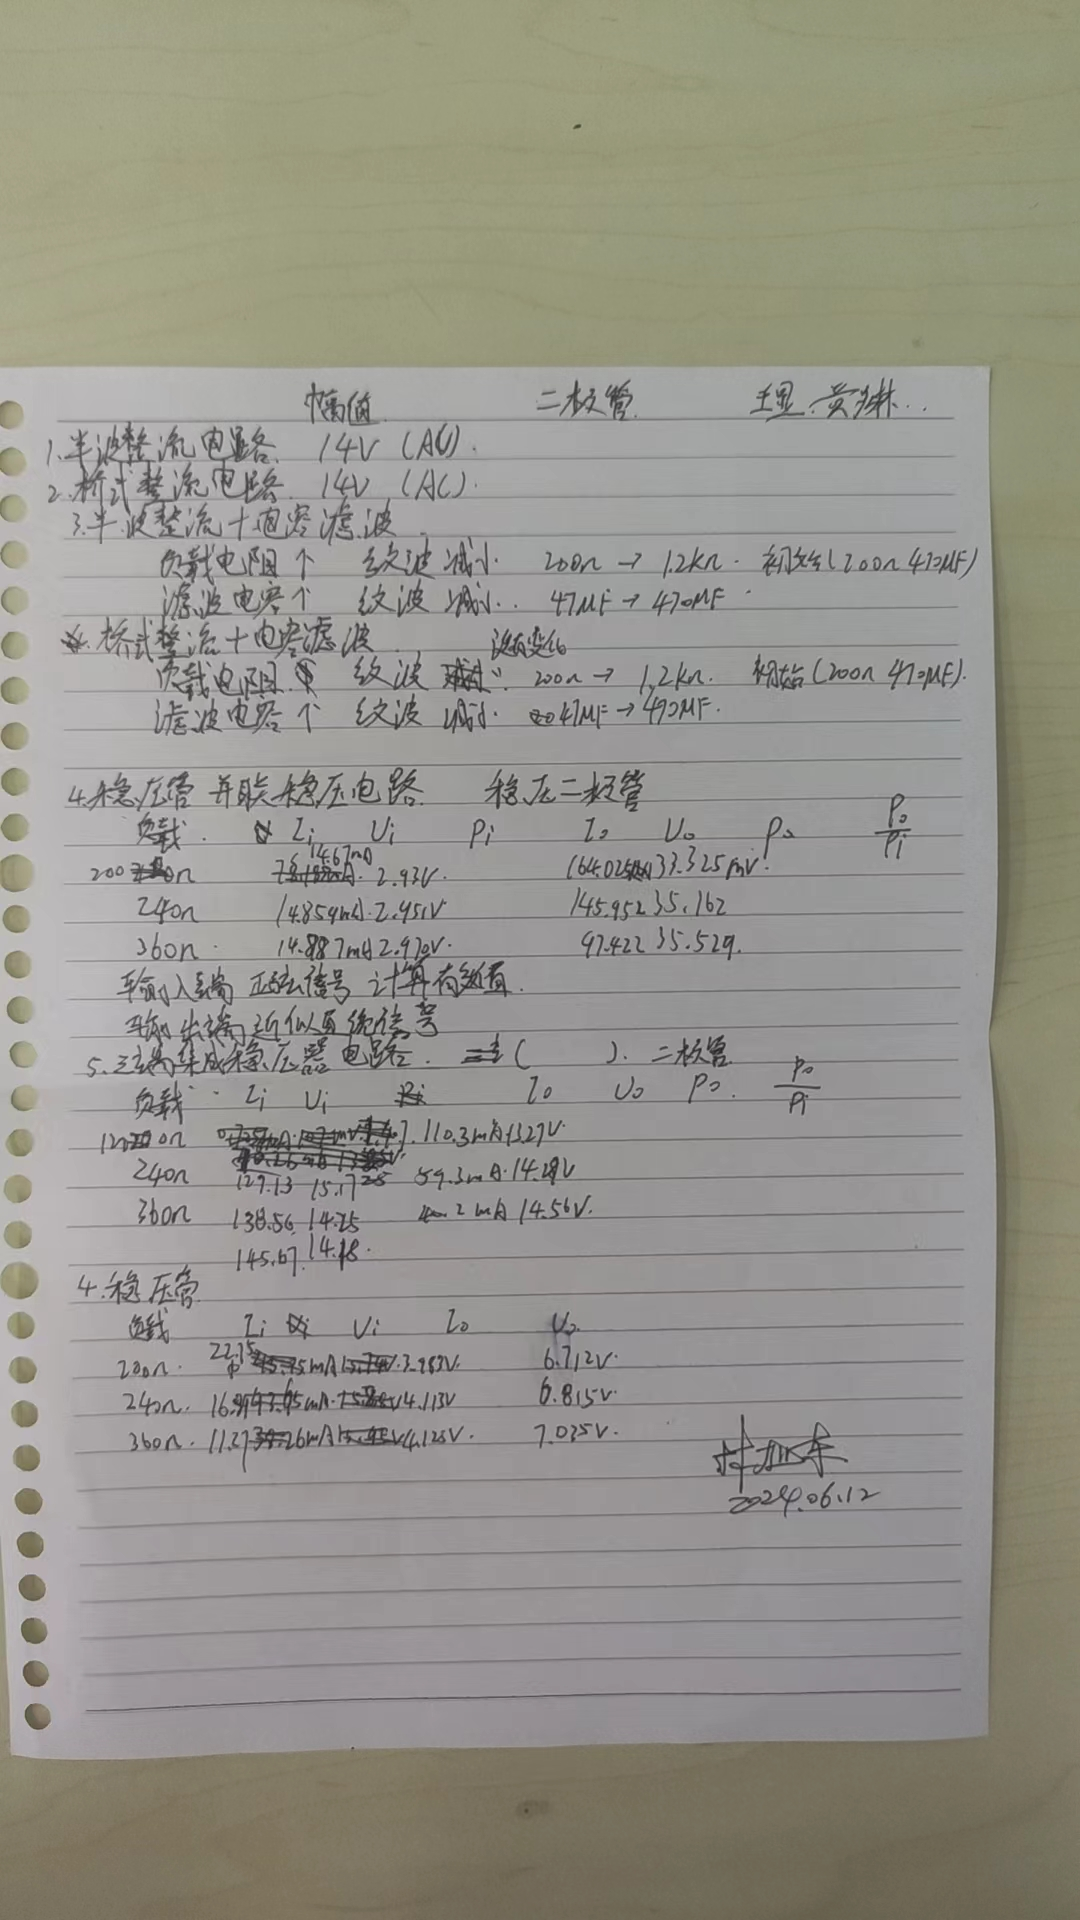
\includegraphics[width=0.2\linewidth]{数据.jpg}
		\caption{实验数据}
		\label{}
	\end{figure}
	% ---
	
	
\end{document}